\documentclass[12pt]{article}
\newenvironment*{remerciements}{%
\renewcommand*{\abstractname}{Remerciements}
\begin{abstract}
}{\end{abstract}}
\newenvironment*{conclusion}{%
\renewcommand*{\abstractname}{Conclusion}
\begin{abstract}
}{\end{abstract}}

\renewcommand{\listfigurename}{Liste des figues}
%%%%
\usepackage{titlesec}
\titleformat{\subparagraph}{\normalfont\normalsize\bfseries}{\thesubparagraph}{1em}{}
\titlespacing*{\subparagraph}{\parindent}{3.25ex plus 1ex minus .2ex}{.75ex plus .1ex}

\setcounter{secnumdepth}{5}
\setcounter{tocdepth}{5}


%%%
\usepackage[english]{babel}
\usepackage{natbib}
\usepackage[T1]{fontenc}
\usepackage{url}
\usepackage[utf8x]{inputenc} 
\usepackage{amsmath}
\usepackage{graphicx}
%graphicspath{{images/}}
\usepackage{parskip}
\usepackage{color}
%usepackage{pgf,tikz}
\usepackage{tikz}
\usetikzlibrary{arrows,decorations.pathmorphing,backgrounds,fit,positioning,shapes.symbols,chains}
\usepackage[siunitx]{circuitikz}
\usepackage{float}
%usepackage[small,hang]{caption2}
\usepackage{fancyhdr}

\usepackage{multicol}  % Pour une page en multi-colonnes 
\usepackage{outlines}
\usepackage{vmargin}
\setmarginsrb{2,5 cm}{2 cm}{2,5 cm}{2 cm}{0,5 cm}{1 cm}{0,5 cm}{1 cm}

\title{ Mémoire de fin d'étude }								% Title
\author{Hajar Boulhdir}								% Author
\date{18 Juin 2018}											% Date

\makeatletter
\let\thetitle\@title
\let\theauthor\@author
\let\thedate\@date
\makeatother

%\pagestyle{fancy}
%\fancyhf{}
%\rhead{\theauthor}
\cfoot{\thepage}
%\makeatletter\@addtoreset{chapter}{part}\makeatother
\begin{document}
%biblist.bib
%%%%%%%%%%%%%%%%%%%%%%%%%%%%%%%%%%%%%%%%%%%%%%%%%%%%%%%%%%%%%%%%%%%%%%%%%%%%%%%%%%%%%%%%%
\begin{titlepage}
	\begin{center}
	 \vspace*{0.5 cm}
    \textsc{\LARGE Université Paris Nanterre }\\[1.0 cm]	% University Name
    
\includegraphics[scale = 0.5]{UPN.jpg}
   \vspace{2 cm}
   \\\textsc{\Large Master 2 Méthodes Informatiques Appliquées à la Gestion d'entreprise }\\[0.3 cm]				% Course Code
% Course Name
\vspace{1 cm}
	\rule{\linewidth}{0.2 mm} \\[0.4 cm]
	{ \huge \bfseries \thetitle}\\
    \vspace{0.4cm}
   \Large Comment les données et le data mining pourraient aider un fournisseur de l’énergie à anticiper une négociation ? \\[0.3 cm]
    \rule{\linewidth}{0.2 mm} \\[1.3 cm]
     \textsc{Par:\\ Hajar BOULHDIR}
   
	\end{center}
   
	 \vspace{0.8 cm}
     \begin{flushleft} \large
	%\begin{minipage}{0.4\textwidth}
		
        \emph{Tuteur à l'université :} \\
			François Delbot \\ 
		\emph{Tuteur en entreprise :} \\
			Naïm CHAMI \\  
      \end{flushleft}
	  
          	
	%\end{minipage}~
 
	\begin{center} 
	{\large 19 Juin 2018}\\[2 cm]
	\end{center} 
\fbox{\parbox{\textwidth}{Les données transmises dans ce documents concernant l'étude pratique sont strictement 
\\confidentielles et ne doivent pas être partagées.}}
	\vfill
\end{titlepage}

%%%%%%%%%%%%%%%%%%%%%%%%%%%%%%%%%%%%%%%%%%%%%%%%%%%%%%%%%%%%%%%%%%%%%%%%%%%   PAGE VIERGE   %%%%%%%%%%%%%%%%%%%
\newpage
\strut
\newpage

%\begin{abstract}
%Je r\'esume pour faire court.
%\end{abstract}

%\newpage

\vspace*{\stretch{1}}

\begin{remerciements}

Je tiens à remercier mon directeur de mémoire, François DELBOT et son doctorant Vincent GROLLEMUND pour toute l’aide qu’ils m’ont apporté, le temps qu’ils ont su prendre pour m’aiguiller dans la réalisation de mon mémoire 

Je souhaite remercier mes collègues de l’équipe pricing et plus particulièrement Vincent BLOUZARD l’expert Oracle qui m’a aidé à bien comprendre les différentes bases de données.
Aussi, j’aimerai remercier Jérôme DUPONT, ainsi que mon manager Naïm CHAMI pour leurs conseils, leurs disponibilités et pour leur participation dans l’étude de cas de ce mémoire.

Je tenais sincèrement à remercier tous ceux qui m’ont apportés de l’aide et de la motivation dans la réalisation de ce mémoire.
\newline
\\
\newline
\\
\newline
\\
\newline
\\
\newline
\\
\newline
\\
\newline
\\
\newline
\\
{\raggedright
‘Laissons l’avenir dire la vérité, et évaluer chacun en 
\newline fonction de son travail et de ses accomplissements.Le présent \newline est à eux ; le futur, pour lequel j’ai réellement travaillé, est mien.’  \newline \bf Nikola Tesla 
}
\end{remerciements}

\vspace*{\stretch{1}}

\newpage
\strut


%%%%%%%%%%%%%%%%%%%%%%%%%%%%%%%%%%%%%%%%%%%%%%%%%%%
\newpage

\renewcommand{\contentsname}{Sommaire} % changer l'appellation

\tableofcontents
\pagebreak

\newpage

\renewcommand{\listfigurename}{Liste des figures}

\listoffigures
\pagebreak
%%%%%%%%%%%%%%%%%%%%%%%%%%%%%%%%%%%%%%%%%%%%%%%%%%%%%%%%%%%%%%%%
\newpage
\strut
%%%%%%%%%%%%%%
\vspace{\stretch{1}}

\section{Introduction}
\textbf{\large Mieux comprendre aujourd’hui, c’est prédire demain}


Faire des prédictions et anticiper l’avenir, c’est une envie qui existe sans doute depuis que l’humanité est apparue. L’Homme a toujours cherché des clés pour mieux lire le futur.
Le Big Data, les algorithmes sophistiqués d’analyse de données nous permettent aujourd’hui d’anticiper toujours plus finement de quoi sera fait demain. 
L’analyse prédictive, c’est l’usage statistique des données collectées pour prévoir un comportement sous la forme d’hypothèses valides. Ce type d’analyse ne constitue pas un phénomène entièrement nouveau, mais la forme que prend cette analyse passe des prédictions fondées sur l’expérience, l’intuition et la pensée critique à des prédictions fondées sur l’analyse technologique de données mal ou non exploitées. 

Dans le contexte actuel où le consommateur est considéré comme volatile, où la concurrence s’intensifie et où les marchés deviennent saturés, le client devient l’acteur principal de l’entreprise. 
Un nouvel enjeu stratégique pour les entreprises est donc né: la récolte d’informations et leurs analyses qui permettent d’avoir des renseignements sur leurs environnements et sur leurs évolutions. 

L’information devient alors \textbf{source de revenu et de compétitivité} voire peut être même un moyen organisationnel. Ces données sont \textbf{historisées et analysées afin de suivre l’activité passée et présente, et anticiper les évolutions futures} dans le but de changer les règles du jeu.


\textbf{\large Présentation de la problématique:}

L'idée de  ce sujet de ce mémoire m'est venue lors de mon stage de M1. Durant ce stage, je me suis rendue compte de certaines problématiques auxquelles mon équipe était confrontée, et l'une des principales était le taux de charge de travail élevé lors des périodes de négociations de contrats.

Pour négocier un contrat, les clients lancent des appels d’offres auxquels les commerciaux répondent.
La réponse à un appel d’offre exige un travail important de plusieurs équipes (plusieurs ateliers, enquêtes et études sont mises en place). De mon côté j’ai eu l’occasion de travailler avec les monteurs d’offres qui se chargent d’aider les commerciaux à établir la meilleure combinaison structure de l’offre/prix en fonction du besoin client.

La prédiction de ces périodes de fortes demandes de négociations des contrats permettra alors à la direction de mieux gérer la mise à disposition des ressources humaines nécessaires.
C’est la raison pour laquelle la direction Marketing fixe comme objectif la mise en place d’un outil de prédiction permettant de donner une estimation du nombre de négociations durant ces périodes.

Curieuse de découvrir dans quelles mesures les analyses prédictives peuvent permettre de rester en tête de la compétition vis à vis des autres concurrents, nous proposons dans cette étude d’analyser les différentes méthodes de datamining et de comparer les outils de prédiction du marché afin de proposer une solution avec ces 3 principaux gains:

\begin{enumerate}
\item \textbf{Organisationnel:} bien dimensionner les équipes, recruter ou déplacer les monteurs d'offres sur d'autres missions, éviter les surcharges...

\item \textbf{Financier:} Prédiction des volumes de l'énergie

\item \textbf{Pilotage:} Gestion de plan moyen terme de la direction pour les 3 prochaines années, projection des gains pour qu'on puisse piloter et prendre des décisions.
\end{enumerate}
 \medbreak
\textbf{\large Structure du mémoire:}
 \medbreak
Afin de répondre à ce vaste sujet, nous nous focaliserons dans cette étude sur les axes suivants :

\begin{itemize}
\item L’analyse pour la prédiction et ses concepts
\item Les méthodes théoriques, statistiques et les techniques de datamining de prédiction et du clustering 
\item La comparaison de différentes techniques.
\end{itemize}

Après avoir défini les différents concepts, pré-requis pour la bonne compréhension de cette étude, ces grands principes seront détaillés au travers d'une approche théorique, puis appliqués à une étude de cas concrète d’anticipation de négociation de contrats. Le parallèle entre l'attendu et le constat nous permettra d’apprécier l’intérêt des analyses prédictives dans un tel environnement, tout en apportant des hypothèses d'amélioration sur les problématiques engendrées ou non résolues.


Avec l’aide de nos conclusions comme de nos hypothèses, nous répondrons à la problématique initiale de cette étude tout en offrant une ouverture sur les aspects de la prédiction qui demeurent encore inexplorés.

\pagebreak
%%%%%%%%%%% La coupure %%%%%%%%%

\section{Etat de l’art :}
\subsection{Achat industriel, négociation et comportement des clients}
\subsubsection{Achat industriel:}

Avant de donner une définition d’un “achat”, il est nécessaire de mettre l’accent sur l’acte d’achat.

Il existe tout d’abord le \textbf{"Business to Customer", "B to one" ou "B to C"}  qui désignent les achats effectués par les consommateurs finaux ou particuliers pour leur consommation personnelle. Dans ce cadre, les entreprises proposent des produits et services aux individus, soit en réponse à un besoin manifesté, soit en prévision d'un besoin, ou encore en créant un nouveau besoin.
Le deuxième type d’achat \textbf{"Business to business" ou “B to B”,} qui correspondent aux achats effectués par les entreprises qui acquièrent des biens et services en vue de produire d'autres biens et services. Il s'agit là d'une démarche en amont au sein de toutes les entreprises qui se veulent compétitives et qui aboutissent à une forme nouvelle de marketing appelé marketing achats. 
C'est précisément cette dernière catégorie d'achats qui nous préoccupe et qui fera l'objet de notre réflexion dans le cadre de ce travail.

Alors, c’est quoi \textbf{un achat?}

Selon J.P Durand, "l'achat désigne l’acte qui consiste à acquérir un service ou un produit, moyennant une contrepartie financière" {\color{red}[Durand 1995]}. Notant que sur le marché industriel, l’acte d’achat ne fait pas forcément référence aux achats pour des fins de produire d’autres biens et services mais également tous les types d’achats avec toutes les fins tant que c’est contre une partie financière.

Considérant qu’il y a plusieurs types d’entreprises (petites, moyennes et grandes) chacune avec sa propre politique et stratégie d’achat, on peut donc dire que le volume et la qualité des achats et aussi les méthodes d’approvisionnement varient selon la taille et le poids de ces entreprises, ce qui donne un aperçu sur la complexité de l’acte de l’achat et qui nous laisse dire que les décisions prises par les acheteurs dépendent entre autre de la situation rencontrée.

Il existe 3 types d’achats dans le secteur industriel:
\begin{itemize}
\item \textbf{ Le simple rachat:} ce qui est issue de la routine quotidienne, on repasse les mêmes commandes en modifiant uniquement le volume ou la quantité. 
\item \textbf{Le rachat modifié:} comme le premier, on repasse les mêmes commandes mais en modifiant quelques caractéristiques qui nous semble importantes vis à vis du produit ou du service.
\item \textbf{Les nouveaux achats:} qui sont plus élaborés et qui obéissent à des stratégies et des démarches particulières.
\end{itemize}

La fonction achat est donc le fournisseur attitré de l'entreprise. En d'autre termes elle doit répondre au mieux et au plus vite aux besoins de ses clients internes (les autres services de l'entreprise). Elle consiste à “prospecter les marchés, négocier et sélectionner les produits ou les services répondants aux besoins internes ou externes de l'entreprise”.

Depuis les années 1960, la mise en pratique, s’inspire de l’approche AIDA (Attention, Intérêt, Désir, Action) attribuée au publicitaire américain Elias 'St. Elmo Lewis (1872-1948) et rapportée par Edward K. Strong, Jr. (1884-1963) dans son ouvrage The Psychology of Selling and Advertising.
\medbreak
Les étapes clés des processus achat sont définies comme suit:
\begin{outline}
\1 Identification du besoin
\1	Examen et formalisation du besoin : écriture du cahier des charges
   \2Quels sont les besoins de l'entreprise : volumes, spécifications techniques, niveau de service attendu, lieux de livraison, etc. ?
\1 Analyse du marché:
\2Quels sont les fournisseurs ? Dans quels pays sont-ils localisés ?
\2Quel est leur processus de fabrication ?
\2Quels sont les principaux facteurs de coûts ?
\2Quel est le rapport entre offre et demande ?
\1Rédaction de l'appel d'offres
\1Dépouillement des offres et analyse des résultats
\1Analyse des forces/ faiblesses de chacune des parties
\1Sélection "short list"
\1Négociation (recherche de l'accord) Celui-ci peut se faire en face en face, ou de plus en plus grâce à des outils Internet, du type enchère inversée
\1Contractualisation

\end{outline}

Dans quelques marchés les processus ne s’arrêtent pas ici. Une étape de renégociation s’ajoute, où notre client devient de nouveau un prospect qu’on veut garder.
Dans cette étude, on va s'intéresser à ce processus de renégociation et plus particulièrement dans le secteur de l’énergie.

\subsubsection{Les facteurs influençants la fonction achat: approche basée sur l'observation}
\textbf{\large Facteurs internes:}

Quelques facteurs internes ont déjà été présentés précédemment:
\begin{outline}
\1 Taille et poids de l’entreprise
\1 Types de l’entreprise:
\2 Particulier et professionnel (petits sites)
\2 Professionnel (sites moyens)
\2 Professionnel (sites moyens et grands sites)
\1 Volume qui satisfait son besoin 
\1 Situation de l’entreprise
\end{outline}
Le reste des facteurs sera identifié après une étude statistique sur un échantillon qui m’a été mis à disposition.

\textbf{\large Facteurs externes:}

\textbf{\underline{Concurrence et prix de marché de l'énergie}}

Une bourse (place de marché centralisée) est un lieu de rencontres entre offre (vendeur) et demande (acheteur) d’un certain bien. 
Mais dans le marché de l'énergie plus particulièrement de l’électricité, les bourses électriques sont facultatives, car elles proposent des produits standardisés : blocs horaires pour le lendemain, produits à terme (mois, trimestres, années, base/pointe). Il est à noter que ces bourses ne traitent qu’une fraction des transactions (10\% en France, 65\% en Scandinavie). 
Selon {{\color{red}[PINON 2015]} le marché de l’électricité peut être décomposé en 4 quatre pôles bien distincts:
\begin{outline}
\1 \textbf{La production:} Il s’agit de la “création” de l’électricité par 
\2 des centrales-thermiques (nucléaire, pétrole, charbon, gaz) 
\2 hydroélectriques
\2 par des panneaux solaires ou au moyen de l’énergie éolienne Il peut s’agir également de l’import et d’export de ces énergies.
\1 \textbf{Le transport:} il s’agit du transport de l’électricité sur de longues distances et à des niveaux de très haute tension (THT) 

\1 \textbf{La distribution :} Il s’agit de l’acheminement de l’électricité vers le consommateur final, à un niveau local et sur des lignes de moyenne et de basse tension (la tension de l’électricité est en effet abaissée pour pouvoir être distribuée)

\1 \textbf{La commercialisation ou la fourniture:} Il s’agit de l’achat et de la vente au détail de l’électricité au consommateur particulier ou professionnel.
\end{outline}

Le pôle commercialisation n’est plus un monopole d’EDF vu que les fournisseurs alternatifs peuvent proposer des offres.

En 1er Juillet 2007, les marchés de l’électricité et du gaz ont été ouverts à la concurrence et les tarifs réglementés ont été réformés pour rendre leur maintien plus compatible avec les exigences de la concurrence.

Depuis l’ouverture à la concurrence des marchés de l’électricité, deux Types de contrats coexistent:
\begin{outline}
\1 Contrats aux tarifs réglementés: dont les tarifs sont fixés par arrêté ministériel.
Ce type d’offres n’est proposé que par les fournisseurs historiques sur les territoires de desserte. Seuls EDF pour l’électricité peuvent donc proposer ces tarifs à la souscription. 
\1 Contrats en offre de marché sont des formules dont les prix sont libres et fixés dans le contrat conclu entre le fournisseur et le consommateur. Ces contrats sont proposés à la fois par les fournisseurs historiques (en complément des tarifs réglementés qu’ils proposent) et par les fournisseurs alternatifs qui ne peuvent proposer que ce type de contrats. 
\end{outline}
Au-delà de 36 kVa, les tarifs réglementés ont totalement disparus. Ce type de clients correspond à notre cible : les grands clients et grandes entreprises.

Les principaux acteurs en concurrence sont les producteurs, les commercialisateurs (fournisseurs), les traders et les consommateurs qui échangent sur le « marché » au moyen de transactions bilatérales (directement ou via des courtiers ou des plateformes spécialisées), ou en passant par la bourse, comme le montre la figure suivante:


%%%%%%%%%%%%%%%% figure 1 %%%%%%%%%%%%%%

\begin{figure}[H]
	\centering
    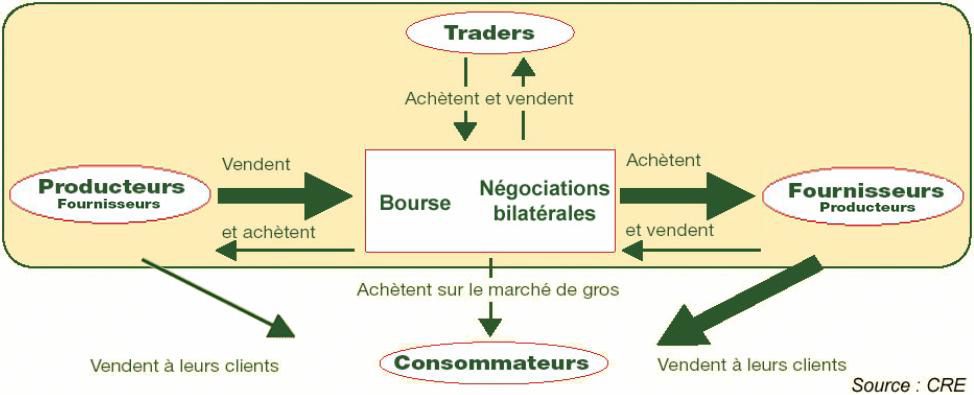
\includegraphics[width=1\textwidth]{image1.png}
     \caption{ Les principaux acteurs du  marché de l’énergie }
    \label{fig:1}
\end{figure}

%%%%%%%%%%%%%%%%%%%%%%%%%%%%%%%%%%%%%%%%

\textbf{\underline{L'\'evolution de la r\'eglementation:}}

L'ouverture du marché de l'énergie avait comme objectif de construire un « marché intérieur de l'énergie » à l'échelle de l'Union européenne. Le but étant de consolider les multiples marchés nationaux à un seul marché européen intégré tout en donnant au consommateur le libre choix de son fournisseur.
La réponse à ces directives européennes a été établie à partir de 1999 comme suit:

\begin{center}
\begin{tabular}{|p{2cm}|p{13cm}|}
\hline
 
  \textbf{Déc 1996} & Première directive européenne sur l'ouverture du marché de l'électricité. \\
  \hline
 \textbf{Fév 1999} & Ouverture du marché pour les entreprises consommant + de 100 GWh. \\
  \hline
  \textbf{Fév 2000} & Ouverture du marché pour les entreprises consommant + de 16 GWh. \\
  \hline
 \textbf{Fév 2003} & Ouverture du marché pour les entreprises consommant + de 7 GWh. \\
  \hline
  \textbf{Août 2004} &	Séparation des activités de production, transport, distribution et fourniture de l'énergie.\\
  \hline
  \textbf{Juil 2004} & Ouverture du marché pour toutes les entreprises et collectivités locales dans toute l'Union Européenne.\\
  \hline
  \textbf{Juil 2007} & Liberté d'établissement des producteurs d'électricité.\\
  \hline
  \textbf{Juil 2007} & Ouverture du marché pour tous les particuliers dans toute l'UE. Fin du monopole d'EDF et GDF, qui se séparent.\\
  \hline
  \textbf{Déc 2010} & Loi NOME : Nouvelle Organisation du Marché de l’Électricité.\\
\hline
\textbf{Jan 2016} & Les tarifs réglementés pour les particuliers sont fixés par la Commission de Régulation de l’Énergie, organisme public indépendant.\\
 \hline
  \textbf{Jan 2016} & Fin des tarifs réglementés pour les entreprises.\\
  \hline
\end{tabular}
\end{center}

 Ce processus se fait au rythme de directives, adoptées par le Parlement européen (PE) avant d'être transposées dans la législation nationale de chaque pays membre. Du fait de la taille du marché et son importance dans la vie des hommes, il est long et fastidieux. Néanmoins, ce processus est déjà bien avancé en France avec un secteur de l'énergie qui s'ouvre de plus en plus chaque année.


\textbf{\underline{La négociation et son impact sur le vendeur: le cas d’un fournisseur d'énergie.}}

Acheter ou vendre de l'énergie est une fonction assez complexe. Dans le cas des fournisseurs d’électricité, on peut citer les impacts suivants:

\textbf{ 1)  Impact organisationnel:}
Une négociation est un processus qui fait travailler plusieurs équipes
\begin{outline}
\1 Les commerciaux qui ont un contact direct avec le client/prospect 
\1 Les pricers qui essaient de formuler l’offre la plus convenable pour un client/prospect donné selon la structure de l’offre et des prix du marché de la période.
\1 Les juristes, le costing, ...
\end{outline}
Prédire une négociation a donc toute son importance pour prévoir un dimensionnement permettant de surmonter un pic de charges

\textbf{2) Impact financier: }
Prédire une négociation va nous permettre de mieu piloter le sourcing de l'énergie

\textbf{3) Impact sur le pilotage:}
Gestion du plan moyen terme de l'énergéticien pour les prochaines années, projection des gains pour qu'on puisse piloter et prendre des décisions. 

\subsection{Data mining: Segmenter ses clients et prédire une négociation grâce aux données}
\subsubsection{Typologie}

\textbf{Data mining}

L'exploration de données est le processus de recherche et d'analyse des données afin de trouver des informations implicites, mais potentiellement utiles. Cela implique de sélectionner, d'explorer et de modéliser de grandes quantités de données pour découvrir des modèles des informations exploitables, à partir de bases de données volumineuses.
L'exploration de données utilise une vaste famille de méthodes computationnelles qui incluent l'analyse statistique, les arbres de décision, les réseaux de neurones, l'induction et le raffinement de règles, et la visualisation graphique.
Bien que les outils d'exploration de données soient disponibles depuis longtemps, les progrès dans le matériel informatique et logiciels, en particulier des outils exploratoires comme la visualisation de données et neuronale réseaux, ont rendu l'exploration de données plus attrayante et plus pratique. 

Le processus d'exploration de données comprend les étapes suivantes {\color{red}[Bounsaythip 2001]}:
\begin{outline}
\1 formulation du problème
\1 préparation des données
\1 construction des modèles
\1 interprétation et évaluation des résultats
\end{outline}

L'extraction de modèle est un composant important de toute activité d'exploration de données et traite des relations entre sous-ensembles de données. Formellement, un motif est défini
comme {\color{red}[Bounsaythip 2001]} une déclaration S dans L qui décrit les relations entre un sous-ensemble de faits Fs d'un ensemble donné de faits F, avec une certaine certitude C, de sorte que S est plus simple que l’énumération de tous les faits dans Fs.
Les tâches d'exploration de données sont utilisées pour extraire des modèles à partir de grands ensembles de données. Les diverses tâches d'exploration de données peuvent être globalement divisées en six catégories, comme indiqué dans la figure suivante :


%%%%%%%%%%%%%%%% figure 2 %%%%%%%%%%%%%%

\begin{figure}[H]
	\centering
    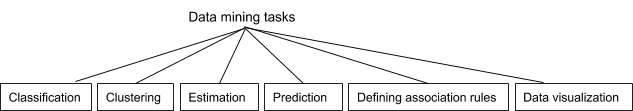
\includegraphics[width=1\textwidth]{image2.png}
     \caption{ Les tâches d'exploration de données }
    \label{fig:2}
\end{figure}

%%%%%%%%%%%%%%%%%%%%%%%%%%%%%%%%%%%%%%%%

La taxonomie reflète le rôle émergent de la visualisation de données en tant que tâche d'exploration de données distincte, même si elle est utilisée pour prendre en charge d'autres tâches d'exploration de données. 
La validation des résultats est également une tâche d'exploration de données. Du fait que la validation supporte les autres tâches d'exploration de données et est toujours nécessaire dans le cadre d'une recherche, cette tâche n'a pas été mentionnée séparément. 
Différentes tâches d'exploration de données sont regroupées en catégories selon le type de connaissances extraites par les tâches. 
L'identification des modèles dans un grand ensemble de données est la première étape pour obtenir des informations marketing utiles et marquer les décisions marketing critiques. Les tâches d'exploration de données génèrent un assortiment de connaissances client et de marché qui constituent le cœur du processus de gestion des connaissances.

Les tâches spécifiques à utiliser dans cette recherche sont \textbf{Clustering} (pour la segmentation des clients), \textbf{Classification} (pour l'estimation du segment), \textbf{Prédiction} (Prédire une négociation) et \textbf{Visualisation} des données.

Typologie des algorithmes {\color{red}[Gorunescu 2011] }


%%%%%%%%%%%%%%%% figure 3 %%%%%%%%%%%%%%

\begin{figure}[H]
	\centering
    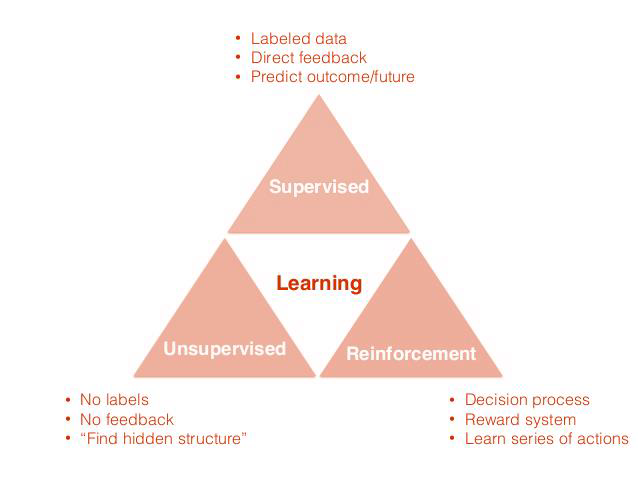
\includegraphics[width=0.7\textwidth]{image3.png}
     \caption{Différents type du machine learning}
    \label{fig:3}
\end{figure}

%%%%%%%%%%%%%%%%%%%%%%%%%%%%%%%%%%%%%%%%
\textbf{Supervisé}

Les algorithmes d'exploration de données supervisés effectuent des prédictions basées sur un ensemble d'exemples. Ce genre d'algorithme cherche des modèles. Une fois que l'algorithme a trouvé le meilleur motif possible, il utilise ce modèle pour faire des prédictions pour les données à prévoir.
Les algorithmes d'apprentissage supervisé sont les algorithmes d'exploration de données les plus populaires, ils sont subdivisés en 3 types d'algorithmes:
\begin{outline}
\1 \underline{Classification:} prédiction de catégorie, peut être multi-classe ou binomiale. Il consiste à étiqueter les données
\1 \underline{Régression:} pour la prédiction de valeur discrète telle que l'évolution du marché boursier
\1 \underline{Détection d'anomalie:} détection de points de données inhabituelle, recherche de variations avec des points de données centrés (habituels)
\end{outline}
\textbf{Non supervisé}

Les techniques d'exploration de données non supervisées varient en ce sens qu'elles n'ont pas d'ensemble d'exemples et en font une auto-intelligence à travers les exécutions. Les données sont automatiquement structurées et regroupées, en prenant des décisions en fonction de l'algorithme utilisé. L'exactitude de la décision prise est mesurée et l'algorithme, comme il est auto-adaptatif, apprendra de ses erreurs et modifiera les décisions suivantes.

\textbf{Apprentissage par renforcement}

En robotique, l'algorithme d'apprentissage par renforcement étudie chaque point de données individuellement, en faisant une action individuelle pour chacun d'entre eux. Ensuite, le résultat de l'action est mesuré et le "robot" adapte sa compréhension de points de données similaires en fonction de l'efficacité des actions précédentes.

\textbf{Sélection des fonctionnalités {\color{red}[Brownlee 2014]}}

La sélection de caractéristiques est la sélection (automatique ou non) d'attributs dans les données (telles que les colonnes dans les données tabulaires) qui pèsent le plus dans le modèle prédictif.
Cette sélection vise à améliorer la précision du modèle en choisissant les caractéristiques qui l'améliorent directement, tout en supprimant les autres contribuant au gain général de précision.

\textbf{Méthodes de filtrage}

Les méthodes de filtrage appliquent des formules statistiques pour évaluer chaque caractéristique. En les classant, l'analyste peut choisir le nombre de fonctionnalités dont il a besoin (par exemple le top 10). Ces méthodes peuvent prendre chaque variable indépendamment ou en regardant l'inter-corrélation.
Quelques exemples de certains filtres: test du Chi au carré, gain d'information et coefficients de corrélation.

\textbf{Méthodes d'emballage}

Les wrappers prennent l'ensemble des fonctionnalités comme une combinaison multiple possible, il va automatiquement évaluer et comparer les différentes combinaisons pour trouver la meilleure. La précision du modèle prédictif est la mesure utilisée pour détecter le meilleur ensemble de fonctionnalités.
Un exemple de méthode wrapper: algorithme récursif d'élimination de caractéristiques.

\textbf{Méthodes intégrées}

Les méthodes intégrées sont présentes dans le modèle prédictif et effectuent la sélection des fonctionnalités à la volée. Dans les algorithmes suivants, nous pouvons considérer les paramètres de régularisation comme des méthodes intégrées.
Exemples d'algorithmes de régularisation: LASSO, Elastic Net et Ridge Regression.

Considérations lors du choix d'un algorithme {\color{red}[Gorunescu 2011]}

\underline{Précision}

La précision n'a pas à être parfaite, car il est parfois plus important de montrer le taux d'erreur que la bonne réponse. Plus un algorithme est précis, plus le risque de surapprentissage apparaît.


\underline{Temps de traitement}

En fonction de l'algorithme choisi, le temps de traitement varie. Il est également lié à la précision, car un modèle plus précis conduit à une consommation de temps plus élevée. La limitation du temps ou de l'architecture peut pousser les développeurs à choisir un modèle moins précis mais plus rapide à exécuter que le modèle parfait, en supposant que la marge avec un modèle plus précis soit un critère de validation.

\underline{Linéarité}

La linéarité signifie que les points de données peuvent être séparés par une ligne droite. En fonction du cas de données, cela peut réduire la précision.


%%%%%%%%%%%%%%%% figure 4 %%%%%%%%%%%%%%

\begin{figure}[H]
	\centering
    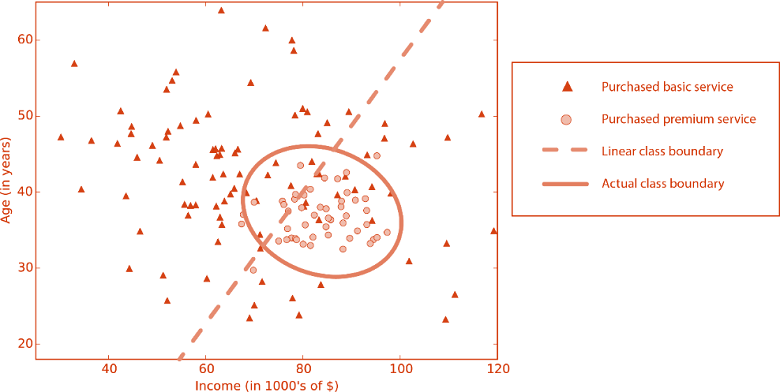
\includegraphics[width=0.70\textwidth]{image4.png}
     \caption{Non linéaire classe boundary}
    \label{fig:4}
\end{figure}

%%%%%%%%%%%%%%%%%%%%%%%%%%%%%%%%%%%%%%%%
%%%%%%%%%%%%%%%% figure 5 %%%%%%%%%%%%%%

\begin{figure}[H]
	\centering
    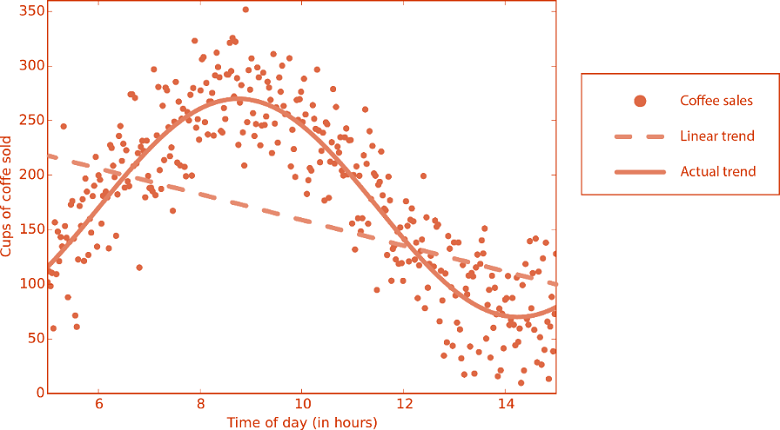
\includegraphics[width=0.65\textwidth]{image5.png}
     \caption{Data with a non linear trend}
    \label{fig:5}
\end{figure}

%%%%%%%%%%%%%%%%%%%%%%%%%%%%%%%%%%%%%%%%
\underline{Nombre de paramètres}

De nombreux paramètres signifient un plus large éventail de possibilités et de solutions pour un algorithme donné. Le travail de l'analyste consiste à trouver la meilleure combinaison de paramètres, c'est ce qu'on appelle le réglage des paramètres. Des solutions existent et automatisent les tests de réglage des paramètres, mais leur utilisation pourrait conduire à des temps d'exécution exponentiels.
\subsubsection{	Segmentation des clients:}
\textbf{C’est quoi le clustering?}

Depuis peu, les analystes commencent à catégoriser les objets en fonction de leurs similitudes. Cette capacité de regrouper les choses aide à comprendre ce que les différents membres d'une population ont en commun et en quoi ils diffèrent des autres. Les data miners ont appliqué cette même approche pour effectuer des clusters. 
Par conséquent, le regroupement consiste à diviser les données en un certain nombre de sous-groupes homogènes au sein du groupe et hétérogènes par rapport aux autres groupes {\color{red}[Berry et Linoff, 2004]}.
De plus, l'analyse de regroupement (clustering analysis) fait référence au processus de découverte automatique des clusters cachés dans les données {\color{red}[Tan, Steinbach et Kumar, 2006]}.
La segmentation est communément utilisée dans le marketing, alors que la classification est beaucoup plus utilisée et ne se limite pas à un domaine d'activité spécifique.
Cependant, dans ce mémoire, ces termes sont utilisés de manière interchangeable.

\textbf{Techniques du clustering}

Dans le domaine de l'exploration de données, plusieurs méthodes existent pour regrouper les données. Deux techniques de clustering couramment utilisées sont connues sous le nom de clustering hiérarchique et partition.

La caractéristique du \textbf{clustering de partition} est que l'ensemble de données doit être divisé en plusieurs clusters dans lesquels chaque échantillon de données ne peut appartenir qu'à un cluster. Pour atteindre cette classification, la classification tente généralement de minimiser la distance au sein des clusters et de la maximiser entre les clusters {\color{red}[Vesanto \& Alhoniemi, 2000].}
%%%%%%%%%%%%%%%% figure 5 %%%%%%%%%%%%%%

\begin{figure}[H]
	\centering
    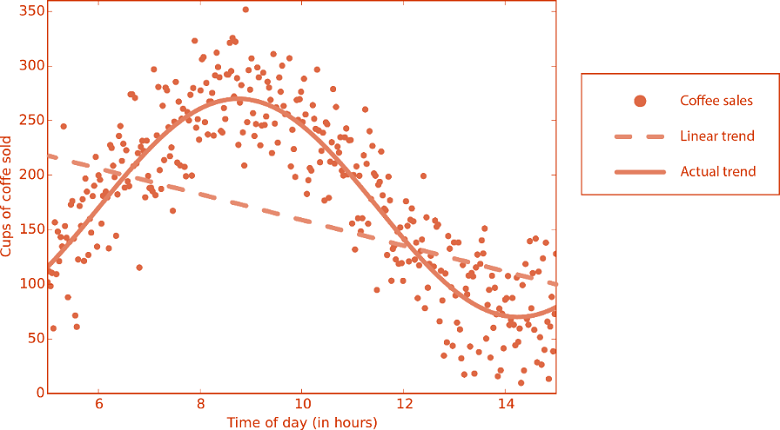
\includegraphics[width=0.55\textwidth]{image5.png}
     \caption{ Clustering de partition [1]}
    \label{fig:5}
\end{figure}

%%%%%%%%%%%%%%%%%%%%%%%%%%%%%%%%%%%%%%%%

D'un autre côté, le \textbf{clustering hiérarchique} consiste à diviser les données à plusieurs reprises en sous-groupes. Lors de la mise en cluster hiérarchique, les objets sont triés dans une arborescence où chaque nœud représente un cluster. La classification hiérarchique peut être effectuée de haut en bas ou de bas en haut {\color{red}[Vesanto,2006]}. Cette dernière approche est mieux connue sous le nom de clustering agglomératif où tous les objets de données sont initialement considérés comme cluster et à chaque étape fusionnés avec le cluster le plus proche. La première approche part d'un nœud racine qui représente tout l'ensemble de données en un seul cluster et divise itérativement les clusters en plus petits {\color{red}[Vesanto,2006]}.

%%%%%%%%%%%%%%%% figure 6 %%%%%%%%%%%%%%

\begin{figure}[H]
	\centering
    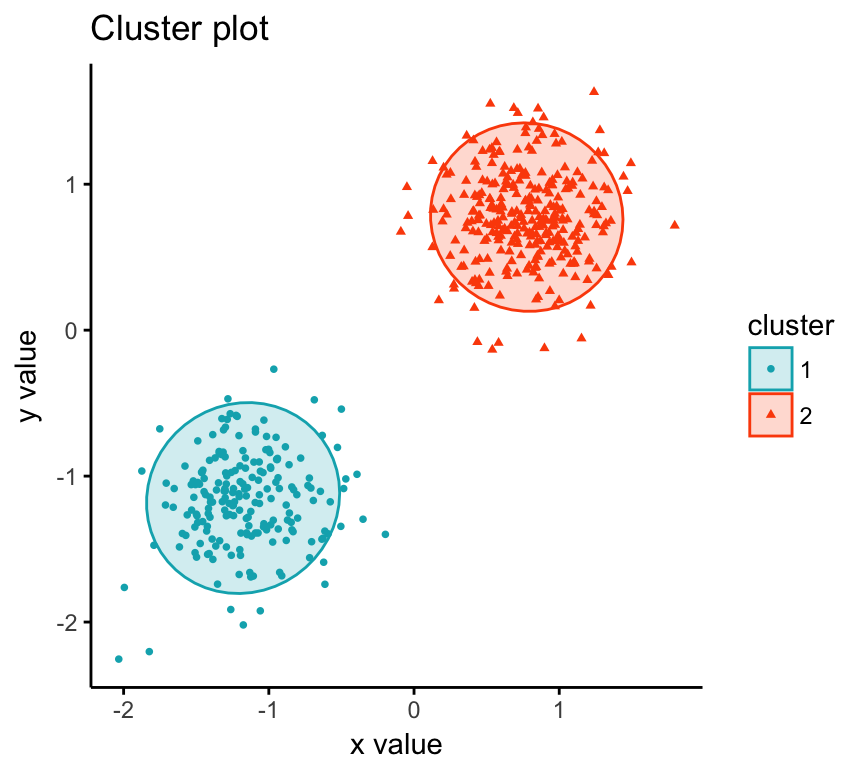
\includegraphics[width=0.6\textwidth]{image6.png}
     \caption{ Clustering hiérarchique [2]}
    \label{fig:6}
\end{figure}

%%%%%%%%%%%%%%%%%%%%%%%%%%%%%%%%%%%%%%%%

D'autres techniques de regroupement existent également, telles que les modèles de mélange et la mise en grappes floue. Les modèles de mélange présentent les clusters comme des distributions où chaque échantillon de données appartient à un cluster basé sur une distribution de probabilité calculée.
Le défi pour ce type de clustering est de savoir comment trouver mathématiquement les paramètres qui décrivent le mieux le cluster. Une faiblesse considérable de la partition et de la classification hiérarchique par rapport au modèle de mélange est qu'ils ne parviennent pas à trouver des groupes qui se chevauchent {\color{red}[Arnborg, 2008]}. 
Dans le clustering flou, chaque échantillon de données a une relation avec chaque cluster décrit comme un poids d'appartenance allant de 0 à 1. Par conséquent, le clustering flou diffère du clustering de partition puisqu'il affecte chaque échantillon de données à tous les clusters avec un poids {\color{red}[Tan, Steinbach, \& Kumar, 2006]} 
Pour simplifier l'analyse effectuée dans ce mémoire, chaque échantillon de données est supposé appartenir à un cluster à la fois.
Lorsque l'on considère quelle technique de regroupement choisir l'aspect le plus restrictif de la classification hiérarchique est la complexité temporelle quadratique O (n2), où n est le nombre d'échantillons de données, alors que la classification par partition a une complexité temporelle linéaire. Par conséquent, en particulier lorsque les ensembles de données sont volumineux, le clustering de partition est considéré comme supérieur au clustering hiérarchique dans les performances de calcul. En outre, le clustering de partition a un avantage sur le clustering hiérarchique qui ne dépend pas des clusters précédemment trouvés {\color{red}[Vesanto \& Alhoniemi, 2000]}.
Le clustering hiérarchique est connu pour former des clusters de meilleure qualité alors que le clustering de partition est plus efficace dans la gestion du bruit {\color{red}[Jain, Murty, \& Flynn, 1999]}. Le grand ensemble de données impose des considérations de performance et, par conséquent, le clustering de partition linéaire est pris en compte dans ce domaine de problème.

\textbf{Problèmes liés au clustering}

Plusieurs facteurs liés à la mise en cluster existent, qui doivent être pris en compte lors du suivi du processus d'exploration de données et de la mise en cluster. Ce sont la qualité des données (erreurs de mesure, bruit, valeurs manquantes, valeurs aberrantes, données en double), le prétraitement (agrégation, échantillonnage et réduction de la dimension) et la compréhension des données (statistiques récapitulatives et visualisation). Les questions suivantes sont considérées comme les facteurs les plus pertinents aux fins de ce mémoire.


\textbf{Méthodes d'analyse de clustering}

Plusieurs algorithmes existent pour des fins de regroupement {\color{red}[Jain et Dubes, 1988]}. Certains d'entre eux sont basés sur l'apprentissage supervisé tandis que d'autres sur l'apprentissage non supervisé. La différence entre ceux-ci est que l'apprentissage supervisé utilise un ou plusieurs ensembles de formation de données groupés manuellement (ou autrement), tels que des étiquettes, afin d'assigner de nouveaux membres à des groupes. D'autre part, l'apprentissage non supervisé trouve les modèles sous-jacents de l'ensemble de données de manière autonome et les propose comme des clusters. Self organizing map et K-means sont basées sur un apprentissage non supervisé tandis que le support vector clustering est un processus d'apprentissage supervisé.

\textbf{Exemples d'algorithmes d'exploration de données pour le partitionnement de données (ou data clustering )}

\underline{K-means} {\color{red}[Berry et Linoff, 2004]}

K-means est l'une des techniques de clustering les plus utilisées. Le K fait référence au nombre de clusters que la méthode trouvera. Les groupes pour les Kmeans sont basés sur la proximité des échantillons de données entre eux  {\color{red}[Berry et Linoff, 2004]}.
K-means est basé sur la recherche des points centraux du cluster en calculant la moyenne d'un groupe d'échantillons de données. K-means construit les clusters en trois phases qui sont décrites dans la figure 3. Pendant la première phase, les K centres de cluster initiaux sont générés aléatoirement. La deuxième phase comprend plusieurs étapes itératives au cours desquelles la distance entre chaque échantillon de données et les centres de cluster est calculée. L'échantillon de données est toujours affecté à son centre le plus proche. La troisième et dernière phase recalcule les centres de clusters en tant que moyenne de tous les échantillons de données du groupe et c'est ainsi que naissent les nouveaux centres. Le processus se poursuit entre la deuxième et la troisième phase et se termine une fois que les centres de cluster ne changent plus. 
Le but de ces phases est de minimiser la somme des erreurs au carré. Plus le taux d'erreur est faible, meilleure est la qualité des clusters.  {\color{red}[Tan, Steinbach et Kumar, 2006]}


Les étapes itératives de K-means pour trouver quatre clusters sont comme suit:

%%%%%%%%%%%%%%%% figure 8 %%%%%%%%%%%%%%

\begin{figure}[H]
	\centering
    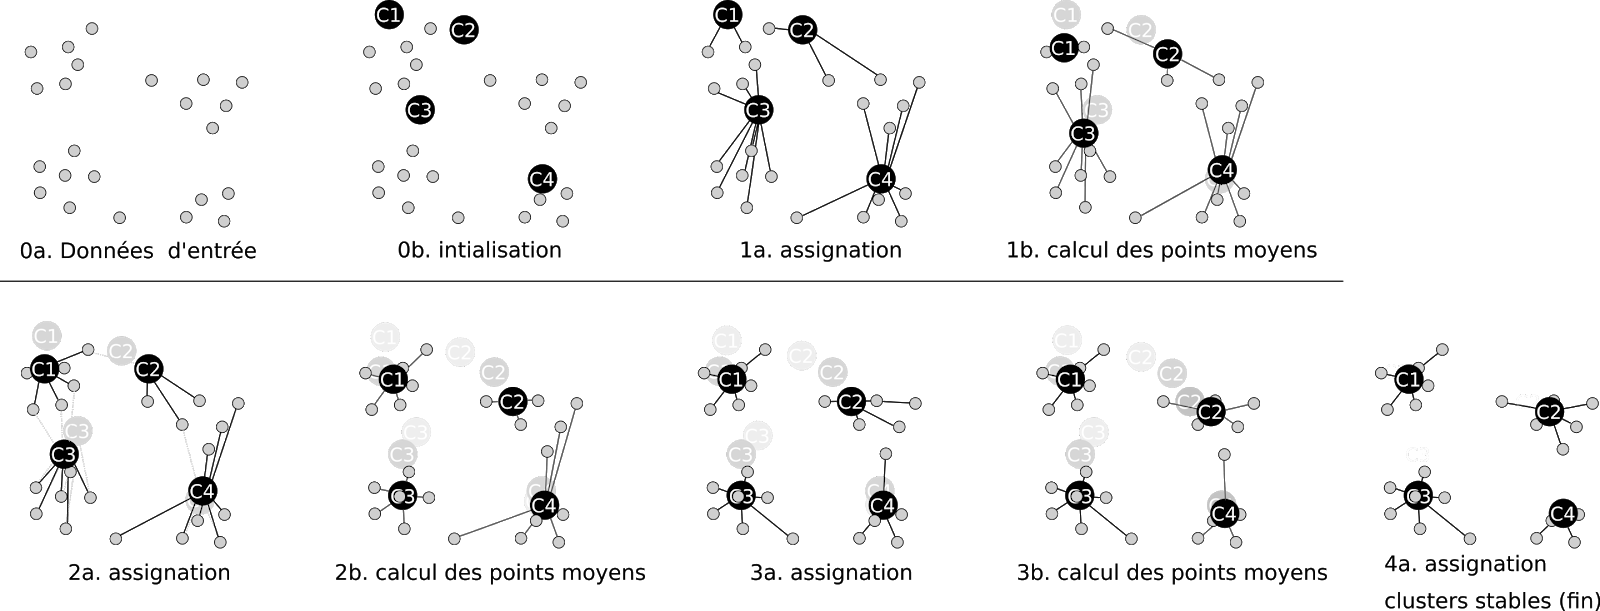
\includegraphics[width=1\textwidth]{image8.png}
     \caption{Les étapes itératives de K-means [Wikipedia]}
    \label{fig:8}
\end{figure}

%%%%%%%%%%%%%%%%%%%%%%%%%%%%%%%%%%%%%%%%
\underline{Self-organizing map}

The self-organizing map (SOM) {\color{red}[Kohonen, Self-organizing map, 1995]} est un algorithme de réseau neuronal basé sur un apprentissage compétitif non supervisé.

À travers l'analyse de la littérature pertinente {\color{red}[Kiang, Hu et Fisher, 2006]},{\color{red}[ Vellido, Lisboa et Meehan, 1999]}, {\color{red}[Hsieh, 2004]}, {\color{red}[Merkevičius, Garšva et Simutis, 2004]}, on peut identifier que la méthode SOM a été largement utilisée dans le domaine de la segmentation. 
En outre, plusieurs types de SOM peuvent être trouvés mais ce mémoire se concentre sur le basique SOM.

Les réseaux de neurones, comme SOM, consistent en un ensemble de nœuds. Le travail de ces nœuds est de prendre des entrées et de les combiner en une seule valeur, qui est ensuite transformée pour produire une sortie. Typiquement, chaque entrée a son propre poids et le nœud forme une somme pondérée de ces entrées, c'est-à-dire que chaque entrée est multipliée par son propre poids et toutes ces valeurs sont additionnées. Pour les réseaux de neurones, les poids sont importants car ils sont utilisés comme paramètres pour résoudre le problème de regroupement.

La structure d'un basique SOM est celle qui a une couche d'entrée et une couche de sortie. Ce que fait SOM, c'est de fournir les échantillons de données pour la couche d'entrée qui ne fait aucun travail mais qui agit seulement comme une connexion pour les attributs d'entrée. Comme on peut le voir sur la figure suivante, chaque attribut d'un échantillon de données (par exemple revenu moyen par mois et nombre de visites par service et occasion de visites par service) est connecté à un nœud sur la couche d'entrée. Cependant, chaque nœud de la couche d'entrée est connecté à tous les nœuds de la couche de sortie. La couche de sortie ressemble à un échiquier mais les nœuds sur la couche de sortie ne sont pas connectés les uns aux autres. La couche de sortie est également connue sous le nom de carte de caractéristiques (feature map) car elle décrit les attributs communs, c'est-à-dire les caractéristiques des données d'entrée sous-jacentes.
%%%%%%%%%%%%%%%% figure 9 %%%%%%%%%%%%%%

\begin{figure}[H]
	\centering
    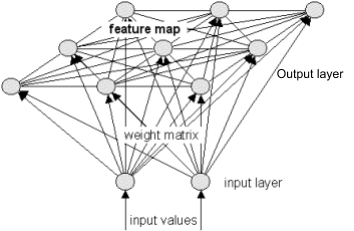
\includegraphics[width=0.75\textwidth]{image9.png}
     \caption{Composantes de SOM  }
    \label{fig:9}
\end{figure}

%%%%%%%%%%%%%%%%%%%%%%%%%%%%%%%%%%%%%%%%
SOM se compose d'une couche d'entrée et de sortie. Chacun des nœuds d'entrée est connecté à un attribut d'un échantillon de données tandis que les nœuds de sortie sont connectés à chacun des nœuds d'entrée. Image de  {\color{red}[Fröhlich, 1997]} avec une petite modification.

Ayant une idée de la structure et des composants, comment se forment les clusters? Imaginez un nid d'abeilles trouvé par des garçons qui commencent à jeter de petites pierres au nid. À chaque coup, une petite bosse est formée sur la surface du nid. Si plusieurs pierres atteignent le même point, un trou est formé. Avec SOM, le nid des abeilles serait la couche de sortie et les trous seraient les groupes.
Pour décrire plus en détail comment les clusters sont trouvés avec SOM, la formation est un concept central. La figure suivante présente la formation des amas lors de la formation. Dans le clustering SOM, les échantillons de données subissent plusieurs cycles de formation. Au cours de chaque tour, on pourrait dire que les nœuds de sortie sont en concurrence les uns avec les autres du droit de posséder les échantillons de données d'entrée. Le nœud gagnant est celui qui décrit le mieux l'échantillon de données d'entrée. En tant que prix, le nœud gagnant obtient de mettre à jour les poids de ses bords d'entrée. Plus le nombre de fois qu'un noeud gagne, il commence à former des modèles et finalement des groupes.

La SOM ne forme pas seulement des groupes, mais elle les forme de sorte qu'ils aient des relations. En pratique, cela signifie que des groupes plus similaires sont plus proches les uns des autres et que la structure sous-jacente des données est préservée. Comment SOM fait cela, que non seulement les poids du nœud gagnant mais aussi ses nœuds voisins sont mis à jour. Plus les nœuds voisins sont éloignés du nœud gagnant, moins ils sont ajustés. Même lorsque les nœuds de sortie ne sont pas directement connectés, la carte modifie toujours la structure à mesure que les nœuds proches sont mis à jour. C'est ce qu'on appelle le concept de voisinage, qui permet à des groupes similaires d'être plus proches les uns des autres et plus éloignés des groupes dissemblables.


%%%%%%%%%%%%%%%% figure 10 %%%%%%%%%%%%%%

\begin{figure}[H]
	\centering
    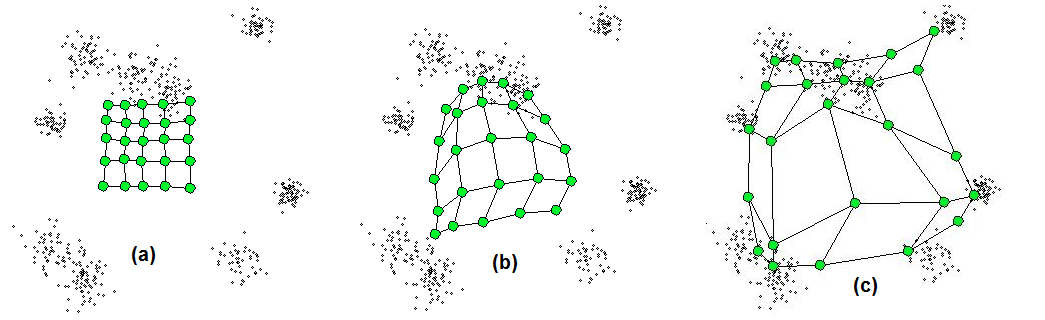
\includegraphics[width=0.9\textwidth]{image10.png}
     \caption{ Calendrier simplifié }
    \label{fig:10}
\end{figure}

%%%%%%%%%%%%%%%%%%%%%%%%%%%%%%%%%%%%%%%%
SOM trouve les clusters cachés à partir des données en ajustant les poids des nœuds et de ses nœuds voisins. (a) Couche de sortie initiale présentée sous la forme d'une carte rectangulaire. (b)
L'entraînement de la carte commence à rapprocher les nœuds gagnants des échantillons de données tout en préservant la structure globale de la carte. (c) Dernière étape de la formation où la carte ne change plus. Les grappes peuvent être identifiées après la fin de l'entraînement. Les images sont des instantanés d'une animation (Peltarion, 2007).

\underline{Support vector clustering}

Une méthode relativement nouvelle que les deux premières mais prometteuse pour la segmentation est le cluster vectoriel de support (SVC). Le SVC est basé sur la théorie des machines à vecteurs de support (SVM)  {\color{red}[Cortes \& Vapnik, 1995]} qui est en fait une technique de classification.

Les machines vectorielles de support sont capables de trouver des modèles (patterns) à partir d'un ensemble complexe d'échantillons de données. Typiquement, ceci est fait en mappant les échantillons de données d'entrée dans un espace de caractéristique de grande dimension où les échantillons sont plus faciles à séparer les uns des autres. Cette méthode a également été appliquée par SVC.

Comment SVC reconnaît-il les modèles (patterns) ? Imaginez que vous regardez un ciel nocturne par une soirée claire. Disons que vous seriez en mesure de sélectionner un ensemble d'étoiles en dessinant un cercle rond dans l'air avec votre doigt. Seule règle pour dessiner le cercle est qu'il doit avoir le plus petit rayon possible qui entoure toutes les étoiles désirées. Ensuite, disons que vous pourriez prendre cette sphère transparente d'étoiles du ciel, la placer sur le sol et piétiner partout. La sphère est maintenant aplatie et comme elle est transparente, vous pouvez voir qu'elle a formé des groupes d'étoiles. Avec un SVC, ces groupes d'étoiles sont les groupes identifiables. La figure 4 montre la sphère et les clusters.

Par conséquent, la première phase de SVC consiste à mapper les échantillons de données d'entrée dans un espace de caractéristiques de grande dimension et un rayon de sphère minimal est calculé qui englobe tous les échantillons de données. C'est comme dessiner le cercle autour de l'ensemble d'étoiles désiré. Tout comme certaines étoiles se trouveront à la surface de la sphère transparente, certains échantillons de données se trouveront également sur la surface. Ceux-ci sont connus comme les vecteurs de support. La seconde phase transforme la sphère en espace de données d'entrée. Après cette phase, la sphère transparente aplatie montre des groupes d'étoiles qui ressemblent à une carte avec des vallées et des sommets. Avec SVC, cela correspond aux vecteurs de support formant des zones de différentes formes. Par conséquent, comme les vecteurs de support sont les points sur la surface de la sphère, ils sont en fait responsables de la formation des limites du cluster. Les échantillons de données à l'intérieur de la sphère se retrouvent dans ces limites.

\subsubsection{Exemples d'algorithmes d'exploration de données pour la prédiction binaire:}

\underline{Perceptron moyen}  {\color{red}[Spoustova 2009]}

Le perceptron est un algorithme d'apprentissage supervisé des classificateurs binaires créé en 1957 par Frank Rosenblatt au Cornell Aeronautical Laboratory, l'un des premiers réseaux de neurones artificiels jamais créés. C'est un algorithme de classification qui fait ses prédictions basées sur une fonction de prédiction linéaire combinant un ensemble de poids avec le vecteur de caractéristiques.
La méthode perceptron moyennée est une méthode d'apprentissage supervisé, c'est une version précoce et très simple de ce réseau neuronal (un seul neurone est représenté).
Les modèles de perceptron moins complexes sont adaptés pour apprendre des exemples directement détachables, bien que les réseaux de neurones (en particulier les réseaux de neurones profonds) puissent modéliser des limites de classes plus complexes. Néanmoins, les perceptrons sont plus rapides que la plupart des réseaux neuronaux. Comme ils traitent les cas en série, ils peuvent être utilisés avec une formation continue.
Dans la plupart des cas, les paramètres sont les suivants:
\begin{itemize}
\item Taux d'apprentissage: taille de l'échelon dans la descente du gradient stochastique à chaque itération du test du modèle. Un taux plus faible induit un nombre élevé de tests, un taux plus élevé fera converger l'exécution plus rapidement avec moins de précision
\item Nombre d'itérations: généralisation à un meilleur ajustement (avec risque de sur-apprentissage)
\item Graine: utilisée pour assurer la reproductibilité de l'expérience dans les essais
\end{itemize}

%%%%%%%%%%%%%%%% figure 11 %%%%%%%%%%%%%%

\begin{figure}[H]
	\centering
    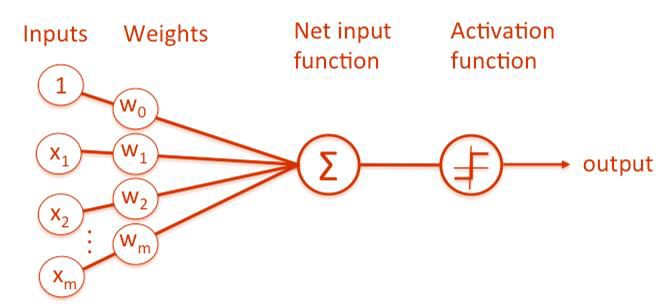
\includegraphics[width=0.7\textwidth]{image11.png}
     \caption{ Schematic perceptron}
    \label{fig:11}
\end{figure}

%%%%%%%%%%%%%%%%%%%%%%%%%%%%%%%%%%%%%%%%

L'algorithme a 4 étapes générales:
\begin{itemize}
\item Recevoir des entrées
\item Entrées de poids
\item Somme des entrées
\item Générer la sortie
\end{itemize}

La sortie est binaire, dans la première machine perceptron c'était l'allumage et l'extinction de l'ampoule.


\underline{Machine à pointer Bayes (BPM)}  {\color{red}[Herbrich 2001]}

BPM est l'un des classificateurs du noyau (kernel-classifiers), ils comprennent une puissante classe de fonctions de décision non-linéaires pour la classification binaire. Il consiste à dessiner une ligne pour séparer les deux classes à prédire. La machine à vecteurs de support (SVM) est une autre option pour cela.
Ils présentent deux algorithmes pour approcher stochastiquement le centre de masse de l'espace de version: un algorithme d'échantillonnage de billard et un algorithme d'échantillonnage basé sur l'algorithme de perceptron. L'approximation stochastique fait référence à l'approximation probabiliste, une technique couramment utilisée dans l'optimisation mathématique. Les erreurs d'entraînement se produisent lorsque les données d'entraînement sont bruyantes ou si le modèle est naïf.
Un classificateur Bayes-optimal est un classificateur qui prédit, pour un point donné, la classe qui minimise l'erreur moyenne lors de la marginalisation sur toutes les limites possibles et tous les échantillonnages possibles des données.
La machine Bayes Point n'est pas sujette à un sur-ajustement des données d'entraînement (training data).
Il améliore la régression linéaire de Bayes sur les parties suivantes:
\begin{itemize}
\item l'algorithme de propagation de message de propagation d'attente est utilisé
\item le balayage des paramètres n'est pas obligatoire
\item les données ne sont pas forcées à être normalisées.
\end{itemize}
Les paramètres sont les suivants:
\begin{itemize}
\item Nombre d'itérations: augmentez la précision en lisant les données d'entraînement plusieurs fois.
\item Biais: caractéristique constante à ajouter à chaque itération (si aucune autre constante n'existe)
\end{itemize}

%%%%%%%%%%%%%%%% figure 12 %%%%%%%%%%%%%%

\begin{figure}[H]
	\centering
    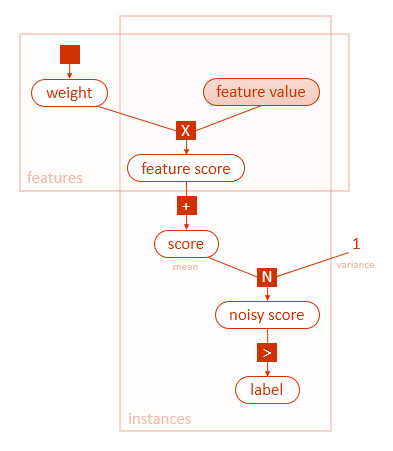
\includegraphics[width=0.5\textwidth]{image12.png}
     \caption{Bayes point machine}
    \label{fig:12}
\end{figure}

%%%%%%%%%%%%%%%%%%%%%%%%%%%%%%%%%%%%%%%%

\underline{ Boosted Decision Tree (BDT)}  {\color{red}[Coadou 2015]}

Le BDT est largement utilisé en sciences sociales, il a commencé par l'exploration de données et la reconnaissance de formes avant de s'utiliser dans des cas concrets.

Il représente un ensemble des méthodes d'apprentissage dans laquelle le deuxième arbre corrige les erreurs du premier arbre, le troisième arbre corrige les erreurs des premier et second arbres, et ainsi de suite. Des prédictions sont ensuite faites sur l'ensemble de l'arbre.
Les BDT utilisent la mémoire de l'ordinateur de manière intensive, ils ne peuvent donc être utilisés que sur de petits jeux de données. Cependant, ils sont faciles à utiliser et à mettre en place.

Les paramètres sont les suivants:

\begin{itemize}
\item Nombre maximum de feuilles par arbre: augmenter donne une meilleure précision, avec un risque de sur-ajustement et un temps de formation plus long
\item Échantillons minimum par nœuds feuilles: augmentation du seuil pour les nouvelles règles, une nouvelle règle est créée lorsque la quantité x de cas similaires est supérieure ou égale à ce paramètre
\item Taux d'apprentissage: de 0 à 1, plus il est petit, plus il est précis, mais l'algorithme prendra plus de temps à s'exécuter
\item Nombre d'arbres: augmenter le nombre d'arbres entraîne une meilleure précision, mais prend plus de temps pour s'exécuter
\item Graine: utilisée pour assurer la reproductibilité de l'expérience dans les essais
\end{itemize}

 %%%%%%%%%%%%%%%% figure 13 %%%%%%%%%%%%%%

\begin{figure}[H]
	\centering
    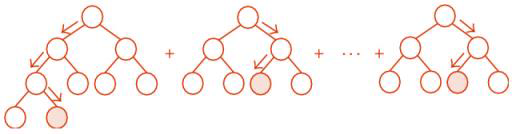
\includegraphics[width=0.8\textwidth]{image13.png}
     \caption{Boosted decision tree additions [Coadou 2015]}
    \label{fig:13}
\end{figure}

%%%%%%%%%%%%%%%%%%%%%%%%%%%%%%%%%%%%%%%%
 
\underline{Forêt de décision} {\color{red}[Chen 2005]}

La forêt de décision est un modèle d'apprentissage automatique basé sur l'algorithme des forêts de décision aléatoires, il est supervisé. Il construit plusieurs arbres de décision, puis sélectionne la classe de sortie la plus populaire. La sélection est faite en agrégeant la fréquence d'apparition de la classe. Ce processus d'agrégation renvoie la probabilité pour chaque classe.

Les arbres de décision sont des modèles non paramétriques et ils renforcent les données avec des distributions fluctuantes.
Les arbres de décision ont de nombreux avantages:
\begin{itemize}
\item Ils peuvent représenter des limites de décision non linéaires.
\item Ils maîtrisent le calcul et l'utilisation de la mémoire pendant l'entraînement et la prédiction.
\item Ils effectuent la sélection et la classification des fonctions intégrées.
\item Ils sont forts dans la vue des caractéristiques tapageuses.
\item Il fonctionne avec compétence sur de grandes bases de données.
\item Il peut gérer un grand nombre de variables d'entrée sans annulation de variables.
\item Il donne des évaluations des facteurs critiques dans la caractérisation.
\item Il dispose d'une stratégie viable pour évaluer les informations manquantes et maintenir la précision lorsqu'une grande partie des données est absente.
\item Il détecte les interactions variables
\end{itemize}
Les paramètres sont les suivants:
\begin{itemize}
\item Méthode de ré-échantillonnage: ensachage (arbres ré-échantillonnés, confiance plus élevée) ou répétition (même intrant, diversification plus élevée)
\item Nombre d'arbres de décision: l'augmentation entraîne une meilleure précision, au prix d'une augmentation du temps de formation
\item Profondeur maximale: augmenter le résultat donne une meilleure précision, au prix d'une augmentation du temps d'entraînement et du sur-ajustement
\item Nombre de divisions aléatoires par nœud: la division est la division aléatoire des différentes entités
\item Nombre d'échantillons par nœud feuille: augmenter le seuil pour les nouvelles règles, une nouvelle règle est créée lorsque la quantité x de cas similaires est supérieure ou égale à ce paramètre
\end{itemize}
 %%%%%%%%%%%%%%%% figure 14 %%%%%%%%%%%%%%

\begin{figure}[H]
	\centering
    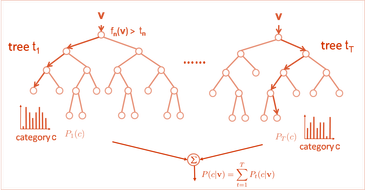
\includegraphics[width=0.8\textwidth]{image14.png}
     \caption{Decision forest [Chen 2005]}
    \label{fig:14}
\end{figure}

%%%%%%%%%%%%%%%%%%%%%%%%%%%%%%%%%%%%%%%%

\underline{Régression logistique} {\color{red}[King 2001]}


La régression logistique est utilisée pour représenter les données et pour clarifier la connexion entre une variable binaire dépendante et une ou plusieurs variables indépendantes nominales, ordinales, d'intervalle ou de rapport. L'algorithme prédit la probabilité d'occurrence d'un événement en ajustant les données à une fonction logistique.
Cet algorithme est une méthode d'apprentissage supervisé.
Les paramètres sont les suivants:
\begin{itemize}
\item Tolérance d'optimisation: seuil qui termine la formation lorsque les itérations cessent de s'améliorer
\item Poids de régularisation L1 / L2: L1 si modèle clairsemé, L2 sinon
\item Taille de la mémoire pour Broyden-Fletcher-Goldfarb-Shanno: moins de mémoire entraîne un entraînement plus rapide mais une précision moindre
\item Graine: utilisée pour assurer la reproductibilité de l'expérience dans les essais
\end{itemize}

 %%%%%%%%%%%%%%%% figure 15 %%%%%%%%%%%%%%

\begin{figure}[H]
	\centering
    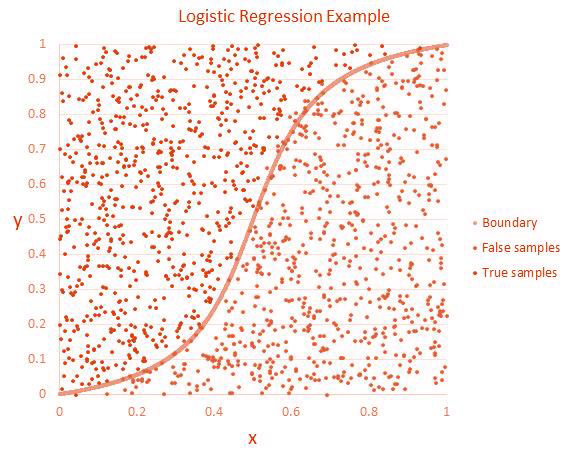
\includegraphics[width=0.7\textwidth]{image15.png}
     \caption{Logistic regression}
    \label{fig:15}
\end{figure}

%%%%%%%%%%%%%%%%%%%%%%%%%%%%%%%%%%%%%%%%

\underline{Réseau neuronal}  {\color{red}[Rowley 1998]}

En 1943, Warren S. McCulloch, un neuroscientifique, et Walter Pitts, un logicien, ont développé le premier modèle conceptuel d'un réseau neuronal artificiel. Dans leur article, "Un calcul logique des idées imminentes dans l'activité nerveuse", ils décrivent l'idée d'un neurone, une cellule solitaire vivant dans un système de cellules qui reçoit des entrées, forme ces sources d'information, et crée une sortie.
Les réseaux de neurones utilisés comme classificateurs sont une méthode d'apprentissage supervisé.
Un réseau de neurones est un agencement de couches interconnectées, dans lequel les entrées conduisent à des sorties par une série de bords et de nœuds pondérés.
En entraînant le réseau de neurones, les poids sur les bords trouvés en utilisant les données d'entrée. Le titre du diagramme est créé à partir des entrées à travers la couche cachée, avec tous les nœuds du graphe connectés par les bords pondérés aux nœuds de la couche suivante.

%%%%%%%%%%%%%%%% figure 16 %%%%%%%%%%%%%%
\begin{figure}[H]
	\centering
    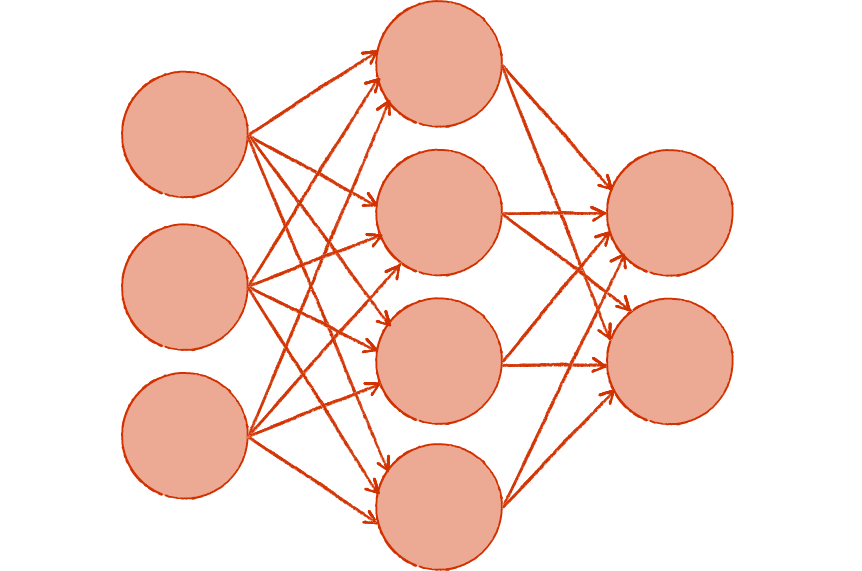
\includegraphics[width=0.5\textwidth]{image16.png}
     \caption{ Neural network }
    \label{fig:16}
\end{figure}

%%%%%%%%%%%%%%%%%%%%%%%%%%%%%%%%%%%%%%%%

Pour acquérir la sortie du réseau pour une entrée donnée, une estimation est calculée pour chaque nœud dans les couches cachées et dans la couche de sortie. Pour chaque nœud, la valeur est établie en calculant la somme pondérée des valeurs des nœuds dans la couche précédente et en appliquant une fonction d'activation à cette somme pondérée.
Les paramètres sont les suivants:
\begin{itemize}
\item Spécification de couche masquée: entièrement connectée (par défaut, une couche masquée) ou personnalisée (à définir par programme)
\item Taux d'apprentissage: la taille de l'étape pour chaque itération, en l'augmentant la fera converger plus vite, mais avec le risque de dépassement de minimum
\item Nombre d'itérations: nombre de formations à exécuter
\item Diamètre initial des poids d'apprentissage: poids du nœud au début du processus d'apprentissage
\item Momentum: poids à appliquer aux nœuds lors de l'apprentissage des itérations précédentes
\item Type de normaliseur: binning (cases de taille égale, division par le total des cases), gaussien (redimensionnement de la valeur avec une moyenne de 0 et variance 1), Min-max (redimensionnement à l'intervalle [0,1]) et non normalisé
\item Shuffle: ordre de cas différent à chaque exécution
\item Graine: utilisée pour assurer la reproductibilité de l'expérience dans les essais
\end{itemize}

\underline{Machine à vecteurs de support (SVM)} {\color{red}[Hearst 1998]}


Comme vu dans le chapitre dernier, les machines vectorielles de support (SVM) sont des modèles d'apprentissage supervisé qui décomposent les données et perçoivent les modèles.
Étant donné un ensemble d'exemples d'apprentissage marqués comme ayant une place dans l'une des deux classes, l'algorithme SVM attribue de nouveaux exemples dans une classification ou l'autre. Les exemples sont représentés comme des points dans l'espace, et ils sont cartographiés de sorte que les cas de la classification différente sont isolés par un espace libre aussi large que possible. Les nouveaux cas sont ensuite cartographiés dans ce même espace et prédits pour appartenir à une classification en fonction du côté de l'écart sur lequel ils tombent.

%%%%%%%%%%%%%%%% figure 17 %%%%%%%%%%%%%%
\begin{figure}[H]
	\centering
    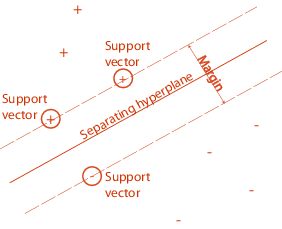
\includegraphics[width=0.5\textwidth]{image17.png}
     \caption{ Support vector machine }
    \label{fig:17}
\end{figure}

%%%%%%%%%%%%%%%%%%%%%%%%%%%%%%%%%%%%%%%%

La feature espace contenant les exemples d'entraînement est appelé hyperplan. Le meilleur hyperplan pour un SVM implique celui avec le plus grand bord entre les deux classes.

Les vecteurs de support sont les points de données les plus proches de l'hyperplan de séparation; ces points sont sur la limite de la dalle.
Les paramètres sont les suivants:

\begin{itemize}
\item Nombre d'itérations: augmentez la précision en lisant les données d'entraînement plusieurs fois.
\item Lambda: coefficient de régularisation
\item Normaliser les caractéristiques: option pour centrer les points de données à la moyenne, avec un écart-type pour chacun d'eux
\item Projet sur la sphère unité: identique à la normalisation, mais pour le coefficient
\item Graine: utilisée pour assurer la reproductibilité de l'expérience dans les essais
\end{itemize}
\newpage
\textbf{Comparaison:}

\begin{center}
\begin{tabular}{|p{3cm}|p{2cm}|p{2cm}|p{2cm}|p{2cm}|p{3cm}|}
\hline
  
  Two-class classification Algorith & Accuracy & Training time & Linearity & Parameters & Notes  \\
  \hline
 logistic regression & & X  & X  &5&  \\
  \hline
  decision forest & X & x & &6 &  \\
  \hline
  boosted decision tree &  X &x& &6&Large memory footprint  \\
  \hline
  neural network & X & & &9&Additional customization is possible\\
  \hline
  averaged perceptron & x &x &X & 4 & \\
  \hline
  support vector machine & &x &X &5&Good for large feature sets   \\
  \hline
   Bayes’ point machine & & x&X &3 &  \\
  \hline
\end{tabular}
\end{center}
%%%%%%%%%%%%%%%% figure 18 %%%%%%%%%%%%%%
\begin{figure}[H]
	\centering
    
     \caption{ Table de Comparaison des algorithmes de prédiction binaire }
    \label{fig:18}
\end{figure}

%%%%%%%%%%%%%%%%%%%%%%%%%%%%%%%%%%%%%%%%

X: mieux que la moyenne

x: pire que la moyenne

\section{Méthodologie de recherche}
\subsection{Objectif:}
Selon {\color{red}[Zhahang et al. 2006]}, le but de la recherche est d'exprimer ce qui devrait être réalisé en menant une recherche et comment les résultats de la recherche peuvent être utilisés. Il peut être classé par son but comme exploratoire, descriptif, explicatif et prédictif. Le but de la recherche exploratoire est de chercher des modèles, des idées ou des hypothèses sous nouvel angle plutôt que de tester ou de soutenir une hypothèse. En outre, la recherche exploratoire peut être menée en utilisant une recherche documentaire, des enquêtes sur les anciennes expériences, des groupes de discussion et des études de cas.
En revanche, la recherche descriptive identifie et obtient des informations sur le profil précis d'une personne ou les caractéristiques d'un problème particulier. Elle est souvent utilisée lorsqu'un problème est bien structuré et qu'il n'y a aucune intention d'étudier la relation cause -effet {\color{red}[Xi Zhang X. et Tang Y, 2006]}.
La recherche analytique ou explicative consiste à comprendre les phénomènes en cherchant et en analysant les relations occasionnelles entre cause - effet. C'est une continuation de la recherche descriptive.
La recherche prédictive va plus loin en prédisant la condition similaire. Le but de cette recherche est de généraliser à partir de l'analyse en prévoyant certains événements sur la base de l'hypothèse. Le tableau suivant montre les différences entre ces trois aspects de la recherche.

\begin{center}
\begin{tabular}{|p{3cm}|p{6cm}|p{6cm}|}
\hline
   Exploratoire& - Pour satisfaire le désir du chercheur d'avoir une compréhension plus claire et meilleure du problème à étudier.
   
- Pour tester la faisabilité d'entreprendre une étude plus approfondie.
 & Quoi, pourquoi et comment une variable produit des changements dans une autre \\
  \hline
   Descriptif&- Décrire et documenter les circonstances et les événements existants  & Quelles sont les actions d'événements visibles, les croyances, la structure sociale et le processus qui se produisent dans ce phénomène? \\
  \hline
   Analytique ou explicatif&- Pour comprendre les phénomènes en recherchant et en analysant les relations occasionnelles entre la cause et l'effet  & Pourquoi et comment une variable provoque des changements dans une autre variable  \\
  \hline
 Prédictif& - Généraliser à partir de l'analyse en prédisant certains événements sur la base de l'hypothèse &  \\
  \hline
  
\end{tabular}
\end{center}
%%%%%%%%%%%%%%%% figure 19 %%%%%%%%%%%%%%
\begin{figure}[H]
	\centering
    
     \caption{ Table des différences entre les aspects de la recherche }
    \label{fig:19}
\end{figure}

%%%%%%%%%%%%%%%%%%%%%%%%%%%%%%%%%%%%%%%%
Ce mémoire a deux buts: descriptif pour un premier lieu et puis prédictif. Les données descriptives seront collectées et analysées afin de nous aider à faire une prédiction.

\subsection{Approches}

Il existe deux approches de recherche principales à choisir lors de la conduite d'une recherche scientifique: quantitative et qualitative {\color{red}[Madani, S., 2009]}. Les approches à utiliser dépendent des caractéristiques des informations collectées et des types de données. En effet, la différence la plus importante entre ces deux approches est la façon dont les données et les statistiques sont utilisées {\color{red}[Wang C. et Wang Zh., 2006]} et aussi en rapport avec le but des questions d'étude et de recherche. La recherche quantitative porte sur les nombres, la logique et l'objectif. Il est basé sur la mesure des variables, la livraison des résultats sous forme numérique et aussi l'analyse menée à travers l'utilisation de diagramme et statistique.
D'autre part, la recherche qualitative se concentre sur la collecte de données non numériques ou l'explication basée sur les attributs du graphique, l'analyse menée à travers l'utilisation de la conceptualisation.
Basé sur des objectifs et des questions de recherche, l'approche choisie pour ce mémoire est l'approche quantitative.
\subsection{Stratégies}
La stratégie de recherche est un plan général de la façon dont les chercheurs vont répondre aux questions de la problématique {\color{red}[Madani, S., 2009]}. Il comprendra un objectif clair issu de ces questions. Elle précise les sources à partir desquelles le chercheur tente de collecter des données et prend en compte l'argent, le temps, l'emplacement et les questions éthiques. Selon {\color{red}[Nosrati, 2008]}, l'identification du type de questions de recherche est la condition la plus importante pour différencier les différentes stratégies de recherche.
Il existe cinq stratégies de recherche en sciences sociales, à savoir l'expérimentation, l'enquête, l'analyse archivistique, l'histoire et l'étude de cas. Le tableau suivant montre chaque stratégie dans les trois conditions et montre comment celles-ci sont liées aux cinq types de stratégies.

\begin{center}
\begin{tabular}{|p{3cm}|p{4cm}|p{4cm}|p{4cm}|}
\hline
   Stratégie& Forme des questions
 & Nécessite un contrôle sur l'événement du comportement &Se concentre sur contemporain \\
  \hline
   Expérimentation&Comment, Pourquoi? & oui &oui\\
  \hline
   Enquête&Qui, quoi, combien, combien?& non &oui\\
  \hline
 Analyse archivistique& Qui, quoi, combien, combien?  & non &non/oui\\
  \hline
   Histoire  &Comment, pourquoi?& non& non \\
    \hline
  Etude de cas  &Comment, pourquoi? & non & oui \\
    \hline
\end{tabular}
\end{center}
%%%%%%%%%%%%%%%% figure 20%%%%%%%%%%%%%%
\begin{figure}[H]
	\centering
    
     \caption{Types de stratégies [Yin, 2003, p.5] }
    \label{fig:20}
\end{figure}

%%%%%%%%%%%%%%%%%%%%%%%%%%%%%%%%%%%%%%%%

La stratégie d'étude de cas est une stratégie courante dans la recherche commerciale qui est généralement associée à une approche quantitative. Elle est basée sur une enquête approfondie d'un individu, d'un groupe ou d'un événement. Une différence fondamentale entre les études de cas et ces méthodes alternatives est que le chercheur de l'étude de cas peut avoir une connaissance moins a priori de ce que seront les variables d'intérêt et comment elles seront mesurées {\color{red}[Benbasa et al, 1987]}.
L'objectif de cette étude est la segmentation des clients afin de prédire par la suite si un client va demander une négociation dans l’avenir ou pas. Les données ont été collectées à partir d'une base de données d’un pricer interne de notre énergéticien. Par conséquent, l'étude de cas est la  stratégie la plus adapté à notre cas. Selon {\color{red}[Benbasa et al, 1987]}, les caractéristiques des études de cas sont comme suit:

\begin{itemize}
\item Le phénomène est examiné dans un cadre naturel.
\item Les données sont collectées par plusieurs moyens.
\item Une ou quelques entités (personne, groupe ou organisation) sont examinées.
\item La complexité de l'unité est étudiée intensivement.
\item Les études de cas sont plus appropriées pour les balises d'exploration, de classification et de développement d'hypothèses du processus de renforcement des connaissances; l'enquêteur devrait avoir une attitude réceptive envers l'exploration.
\item Aucun contrôle expérimental ou manipulation n'est impliqué.
\item L'investigateur ne peut pas spécifier l'ensemble des variables indépendantes et dépendantes à l'avance.
\item  Les résultats obtenus dépendent fortement des pouvoirs intégratifs de l'investigateur.
\item Des changements dans la sélection du site et les méthodes de collecte de données pourraient avoir lieu à mesure que l'investigateur développe de nouvelles hypothèses.
\item La recherche de cas est utile dans l'étude des questions «pourquoi» et «comment» car elles traitent des liens opérationnels à tracer dans le temps plutôt que de la fréquence ou de l'incidence.
\item L'accent est mis sur les événements contemporains.
\end{itemize}

\subsection{Processus du data mining:}
Data Mining (DM) est une technologie permettant de découvrir et d'extraire des informations implicites et utiles à partir de bases de données volumineuses ou d'entrepôts de données. C'est un domaine d'application très apprécié dans la recherche de bases de données. Il peut extraire des connaissances précieuses potentielles, et même des modèles ou des règles réalisables sous une grande quantité de données pour aider les entreprises à trouver des tendances commerciales afin qu'elles puissent faire de meilleures prédictions {\color{red}[Huaping Gong, Qiong Xia, 2009]}. Dans ce projet, notre objectif est d'effectuer la segmentation des clients  afin de prédire une prédiction de négociation par la suite et cela peut être fait par le processus de data mining.

\subsection{Méthodes de collecte de données}
Les données sont la base de la segmentation des clients et la prédiction binaire, il est donc nécessaire de collecter des données relatives et appropriées. Si les données collectées ne sont pas complètes et précises, les étapes de suivi sont totalement inutiles {\color{red}[Cheng Li, 2008]}.
Les données sont classées en tant que données secondaires et données primaires.

Les données secondaires sont collectées à partir de sources secondaires telles qu’une publication; registre personnel et recensement. 

Les données primaires sont recueillies au moyen d'observations, d'entrevues et de questionnaires. {\color{red}[Nosrati L., 2008]} Indique que, en menant une étude de cas en tant qu'étude de recherche, il existe plusieurs sources communes de collecte de données qui peuvent être utilisées. La documentation, les entrevues, l'observation directe, l'observation des participants et les questionnaires font partie des méthodes utilisées pour collecter le maximum de données possible. Le tableau suivant montre la force et la faiblesse de chaque méthode.

\begin{center}
\begin{tabular}{|p{3cm}|p{6cm}|p{6cm}|}
\hline
   Source de données & Points forts & Points faibles \\
  \hline
    Documentation &+ Stable: peut être revu à plusieurs reprises
    
+ Discrète: pas créée à la suite du cas

+ Exact: Contient les noms exacts, les références et les détails d'un événement

+ Large couverture: Longue durée, de nombreux événements et de nombreux paramètres
 & - Récupérabilité: Peut-être faible
 
- Sélectivité biaisée: si la collecte est incomplète

- Biais de reportage: reflète le biais de l'auteur (inconnu)

- Accès: peut-être délibérément bloqué
\\
  \hline
   Dossiers d'archives&+ Pareil que la documentation 
   
+ Précis et quantitatif
& -Pareil que la documentation 

-Accessibilité en raison de la confidentialité bloquée
 \\
  \hline
 Enquêtes& + Ciblé: se concentre directement sur le sujet de l'étude de cas
 
+ Insightful: Fournit des inférences perçues occasionnelles.
 & - Biais dû à des questions mal construites
 
-Biais de réponse

- Inexactitudes dues à un mauvais rappel

-Réflexivité: L'interviewé dit ce que l'interviewer veut entendre

\\
  \hline
   Observations directes  &+ Réalité: Couvrir les événements dans la vraie vie
   
+ Contextuel: Couvre le contexte de l'événement

& - Long

-Sélectivité: Sauf couverture large


-Réflexivité: L'événement peut se dérouler différemment car il est observé

-Cost: beaucoup de temps nécessaire de la part des observateurs humains
 \\
    \hline
  Observations des participants  &+Pareil que l’observation directe
  
+ Perspicace dans le comportement interpersonnel et les motivations
 &-Pareil que l’observation directe
 
-Biais en raison de la manipulation des événements par l'enquêteur

  \\
    \hline
    Artefacts physiques &+ Un aperçu des caractéristiques culturelles

+ Un aperçu des opérations techniques

& -Sélectivité

-Disponibilité
 \\
    \hline
\end{tabular}
\end{center}

%%%%%%%%%%%%%%%% figure 21 %%%%%%%%%%%%%%

\begin{figure}[H]
	\centering
     \caption{ Table de forces et faiblesses des méthodes de collecte de données }
    \label{fig:21}
\end{figure}

%%%%%%%%%%%%%%%%%%%%%%%%%%%%%%%%%%%%%%%%
De nombreuses études utilisent des questionnaires pour la collecte de données. Les questions des questionnaires étaient rarement précisées et, quand elles l'étaient, elles étaient sous une forme très générale. Parfois, les chercheurs mentionnent qu'ils utilisent des documents et des observations, mais ils ne fournissent pas plus de détails à leur sujet {\color{red}[Benbasa et al, 1987]}.
Les données nécessaires à la segmentation des clients et la prédiction dans notre étude de cas ont été fournies par notre énergéticien.


\subsection{Prétraitement des données}

La plupart des données brutes collectées dans la base de données sont imparfaites et bruyantes. Donc, ces données ne sont pas appropriées pour l'exploration de données. Il est nécessaire d'effectuer un prétraitement.
Le prétraitement des données comprend le nettoyage, l'intégration, la sélection et la transformation des données.

\subsection{Nettoyage de données}

Le nettoyage des données est l'une des phases les plus importantes du processus d'exploration de données. Parfois, cela peut prendre beaucoup de temps et être frustrant, mais c'est essentiel pour la recherche quantitative. 
Généralement, si cette phase du projet n'est pas considérée aussi importante que les autres phases, elle montre la faiblesse de la recherche. A ce stade, les erreurs doivent être détectées, les valeurs manquantes doivent être remplies, les champs facultatifs mal conçus ou les attributs inutiles doivent être supprimés et les éléments anormaux ou hors limites ou les éléments ambigus doivent être vérifiés.

\subsection{Transformation de données}

Dans cette étape, les variables du type string “chaîne de caractères” doivent être converties en variables catégorielles numériques ou numériques et certains codes doivent être interprétés ou remplacés par du texte. 

Les autres tâches de cette phase sont l'agrégation de données et la généralisation des données. Dans cette étude, les données des cotations, consommations  d'un client dans une période de temps doivent être agrégées pour effectuer des processus conséquents. 
Dans la généralisation des données, les données de bas niveau seront remplacées par celles de plus haut niveau.

\subsection{Sélection des features et réduction de bruit}

L’Analyse en Composantes principales (ACP) fait partie du groupe des méthodes descriptives multidimensionnelles appelées méthodes factorielles.
Dans la mesure où ce sont des méthodes descriptives, elles ne s’appuient pas sur un modèle probabiliste, mais elles dépendent d’un modèle géométrique.

L’ACP propose, à partir d’un tableau rectangulaire de données comportant les valeurs de p variables quantitatives pour n unités (appelées aussi individus), des représentations géométriques de ces unités et de ces variables. 
Ces données peuvent être issues d’une procédure d’échantillonnage ou bien de l’observation d’une population toute entière. Les représentations des unités permettent de voir s’il existe une structure, non connue a priori, sur cet ensemble d’unités. De façon analogue, les représentations des variables permettent d’étudier les structures de liaisons linéaires sur l’ensemble des variables considérées. 

Ainsi, on cherchera si l’on peut distinguer des groupes dans l’ensemble des unités en regardant quelles sont les unités qui se ressemblent, celles qui se distinguent des autres, etc. Pour les variables, on cherchera quelles sont celles qui sont très corrélées entre elles, celles qui, au contraire ne sont pas corrélées aux autres, etc.

Comme pour toute méthode descriptive, réaliser une ACP n’est pas une fin en soi. L’ACP servira à mieux connaître les données sur lesquelles on travaille, à détecter éventuellement des valeurs suspectes, et aidera à formuler des hypothèses qu’il faudra étudier à l’aide de modèles et d’études statistiques inférentielles. 
On pourra aussi, a posteriori, se servir des représentations fournies par l’ACP pour illustrer certains résultats dans un but pédagogique. {\color{red}[C. Duby, S. Robin]}

Le but d'une analyse en composantes principales est de trouver une nouvelle base orthonormée dans laquelle décrire nos données, de sorte que la variance de ces données, selon les nouveaux axes, soit maximisée.
Voici à quoi cela ressemble en 2D.



%%%%%%%%%%%%%%%% figure 22 %%%%%%%%%%%%%%

\begin{figure}[H]
	\centering
    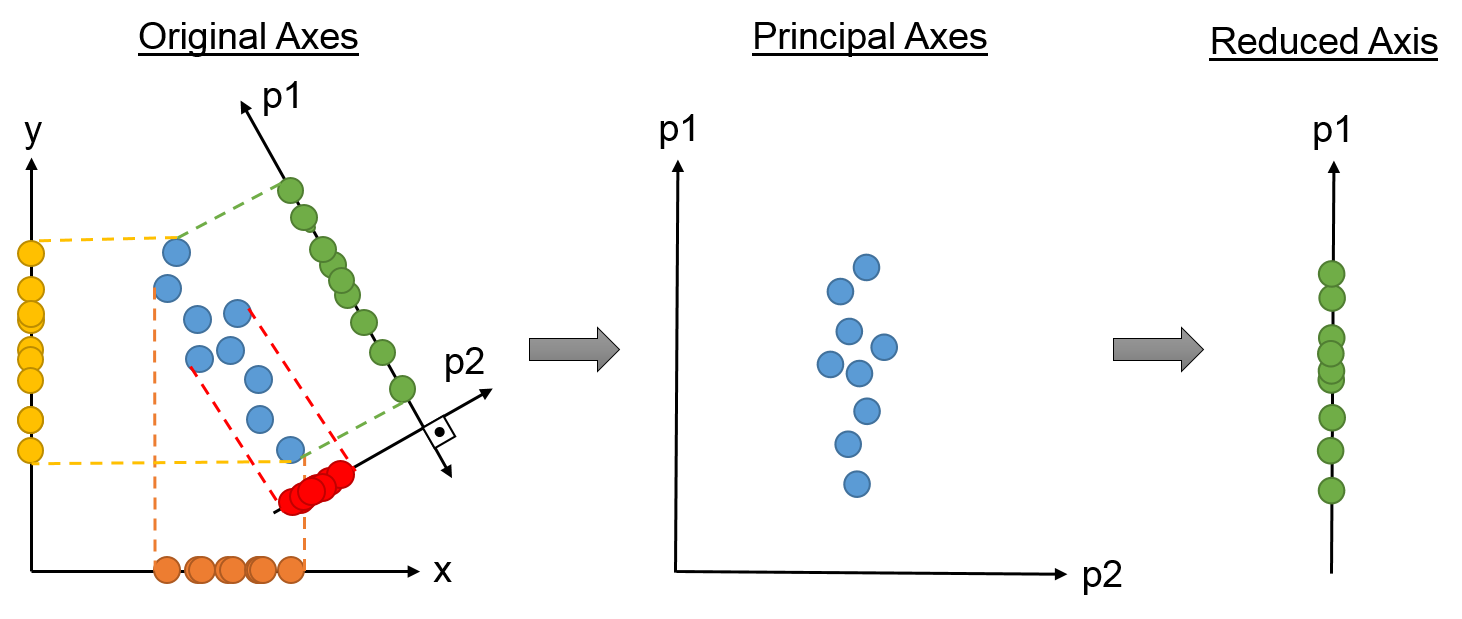
\includegraphics[width=0.8\textwidth]{image22.png}
     \caption{Présentation PCA 2D [Ahmet Cece, 2016] }
    \label{fig:22}
\end{figure}

%%%%%%%%%%%%%%%%%%%%%%%%%%%%%%%%%%%%%%%%

\subsubsection{Clustering de données et segmentation des clients}

Après avoir préparé et optimisé notre base de données et finalement sélectionné les bonnes variables, on peut appliquer les algorithmes de clustering et effectuer des processus conséquents.


\subsection{Prédiction d’une négociation}

Le besoin de notre énergéticien était à la base de prédire si un client va négocier son contrat et quand. Cependant, nous n’avons pu récupérer qu’un échantillon des données pour des raisons évidentes de confidentialité. Avec la volumétrie que l’on a récupérée et l’absence d’autres, notre approche était d’avoir une vision des clients pour qu’on puisse établir une base de règles et voir même prédire les prix de marché pour pouvoir au final prédire une négociation.

 
\section{Résultats et analyse: Énergéticien français, Etude de cas de data mining }
\subsection{Collection et préparation des données}

La première étape (après la formulation du problème) dans le processus d'exploration de données consiste à comprendre les données. Sans une telle compréhension, des applications utiles ne peuvent être développées. 
Les données qu’on a pu récupérer de notre énergéticien sont stockées dans plusieurs bases de données, notamment la base de données d’un pricer d’électricité et une base de données des prix de marché. 
Dans ce chapitre, le processus de collecte des données correctes et complètes sera décrit. 
En outre, le processus de préparation des données pour la segmentation des clients et la prédiction d’une négociation sera explicité.


{\bf Collection des données: Données exportées du Pricer + BD des prix de marché}

Avant chaque négociation, la vente utilise un pricer afin de fixer le prix à proposer à un client donné un jour donné.
La base de données (Oracle) est assez complexe et est composée de plus de 50 tables, les données sont stockées à plusieurs mailles: affaire, ensemble, lot, site et client.

%%%%%%%%%%%%%%%% figure 23 %%%%%%%%%%%%%%

\begin{figure}[H]
	\centering
    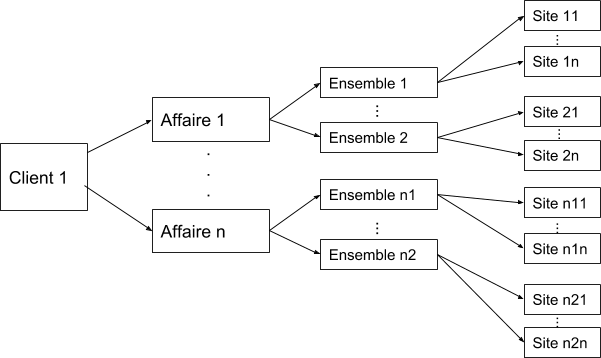
\includegraphics[width=0.6\textwidth]{image23.png}
     \caption{ Logique métier de la BD du pricer }
    \label{fig:23}
\end{figure}

%%%%%%%%%%%%%%%%%%%%%%%%%%%%%%%%%%%%%%%%

Nous disposons d’un échantillon sur un historique de 3 ans avec comme challenge de ne prendre que les champs qui peuvent être utiles pour notre étude. 
Pour cela plusieurs points et réunions avec les experts métiers ont été faites. Plusieurs requêtes d’extraction ont été réalisées pour au final constitué un échantillon représentatif composé de 1543462 lignes. L’historique débute à partir du 12/01/2014 pour se terminer à la date du 24/03/2018.

En raison de la grande confidentialité des données, des colonnes ont été supprimées et d'autres seront supprimées ou anonymisées dans l'expérimentation (comme par exemple les noms des clients). 

Certaines colonnes intéressantes pour identifier un client n’ont pas réellement de sens métier (défaillance code siren) ou vides, on a également rencontré pour le même client des valeurs différentes (erreur humaine lors du remplissage) 

Nous avons listé par la suite la liste des colonnes d’informations susceptible et potentiellement exploitable dans le cas de notre étude:

\begin{center}
\begin{tabular}{|p{6cm}|p{6cm}|}
\hline
Colonne & Importance estimée  \\
  \hline
ID ENSEMBLE & O  \\
  \hline
ID AFFAIRE & O\\
  \hline
ID SITE &O \\
 \hline
PRIX MARCHE& X \\
  \hline
 ID LOT & O \\
\hline
ID SOUS LOT& O \\
    \hline
 ANNEE& X \\
   \hline
 OPTION EEX K& X  \\
  \hline
 OPTION SWAP & X \\
  \hline
 TAUX ARENH  & O \\
  \hline
VOLUME REFERENCE SS LOT &X\\
  \hline
 LIBELLE&O\\
    
    \hline
 FORME PRIX SS LOT&X\\
    \hline
 MARCHE AFF &X\\
   \hline
   SEGMENT COMMERCIAL AFF& X \\
  \hline
 DOMAINE OFFRE&X\\
  \hline
RAE&O\\
  \hline
 TYPE CLIENT SITE&X \\
  \hline
 CODE NAF SITE&O \\
    \hline
SCORE RISQUE LIQUID SITE&X \\
    \hline
MODE RELEVE SITE&X \\
    \hline
    TYPE CONTRAT SITE&X \\
    \hline
   SEGMENT OP RESEAU SITE & X \\
    \hline
   DATE LIVRAISON ENS& X \\
    \hline
   DUREE VALIDITE OFFRE& X \\
    \hline
   VARIANTE& X \\
    \hline
   DUREE CONTRAT&X \\
    \hline
   DATE COTATION& X\\
    \hline
   CONSO SITE&X \\
    \hline
   STATUT LOT&X\\
    \hline
   NOM CLIENT&X \\
    \hline
   NBRSITE &X   \\
    \hline
\end{tabular}
\end{center}

%%%%%%%%%%%%%%%% figure 24 %%%%%%%%%%%%%%

\begin{figure}[H]
	\centering
     \caption{ Table de forces et faiblesses des méthodes de collecte de données }
    \label{fig:24}
\end{figure}

%%%%%%%%%%%%%%%%%%%%%%%%%%%%%%%%%%%%%%%%

{\bf Préparation et nettoyage de données:]}

→ 99.88 \% des données de la colonne prix de marché étaient vides. On a du récupérer, de la base de données prix de marché, le prix journalier moyen de l'électricité pour chaque date de cotation de notre base de données de base

→ Vu qu’un client peut avoir plusieurs codes siren en plus de la défaillance de ces derniers, le seul champ qui reste pour identifier un client est NOM CLIENT. Mais ce champ est rempli manuellement. Du coup, le même client peut être nommé différemment plusieurs fois. La solution était d’utiliser la théorie de distance de Levenshtein pour essayer de retrouver celles qui se ressemblent le plus et corriger l'orthographe. 

\subsection{Analyse et exploration de données:}

Afin de bien comprendre nos données et bien définir notre individu sur lequel on va appliquer les algorithmes de clustering, on peut essayer de visualiser l’évolution de la fréquence des négociations par rapport aux variables numériques ainsi que la répartition des nombres de négociations par rapport aux variables catégorielles (catégories)


-	Evolution des négociations par rapport à :
\begin{itemize}
\item Année de livraison
\end{itemize}
%%%%%%%%%%%%%%%% figure 25 %%%%%%%%%%%%%%

\begin{figure}[H]
	\centering
    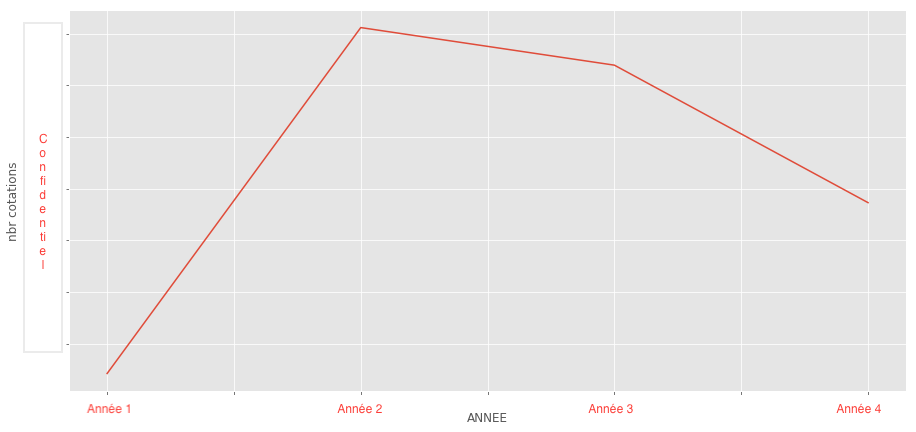
\includegraphics[width=1\textwidth]{image25.png}
     \caption{ Visualisation du nombre de négociation par année }
    \label{fig:25}
\end{figure}

%%%%%%%%%%%%%%%%%%%%%%%%%%%%%%%%%%%%%%%%

{\bf Conclusion 1 :} On observe que pour l'année 2, il y avait un pic de négociations. L'année 2 correspond à une année où le marché de l'énergie a connu une évolution de la réglementation. 

\begin{itemize}
\item Tendance du prix de marché
\end{itemize}

%%%%%%%%%%%%%%%% figure 26 %%%%%%%%%%%%%%

\begin{figure}[H]
	\centering
    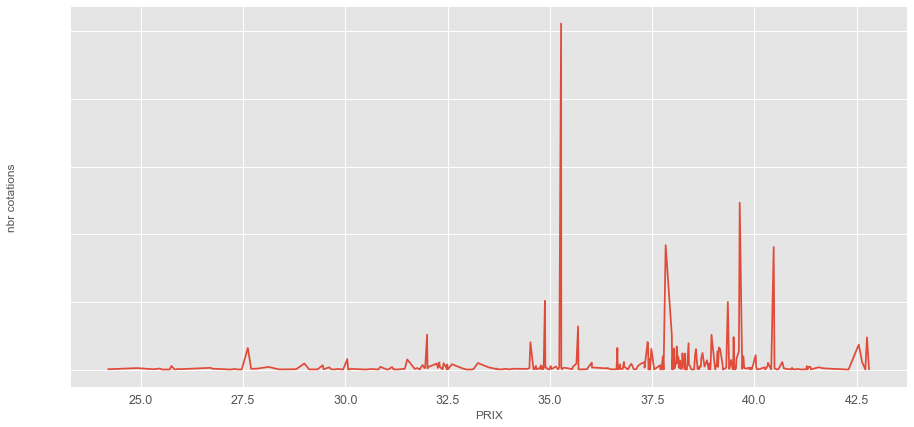
\includegraphics[width=1\textwidth]{image26.png}
     \caption{ Visualisation du nombre de négociations par rapport au prix de marché }
    \label{fig:26}
\end{figure}

%%%%%%%%%%%%%%%%%%%%%%%%%%%%%%%%%%%%%%%%
{\bf Conclusion 2:} Plus le prix de marché augmente plus le nombre de négociations augmentent.

\begin{itemize}
\item Consommation
\end{itemize}

%%%%%%%%%%%%%%%% figure 27 %%%%%%%%%%%%%%

\begin{figure}[H]
	\centering
    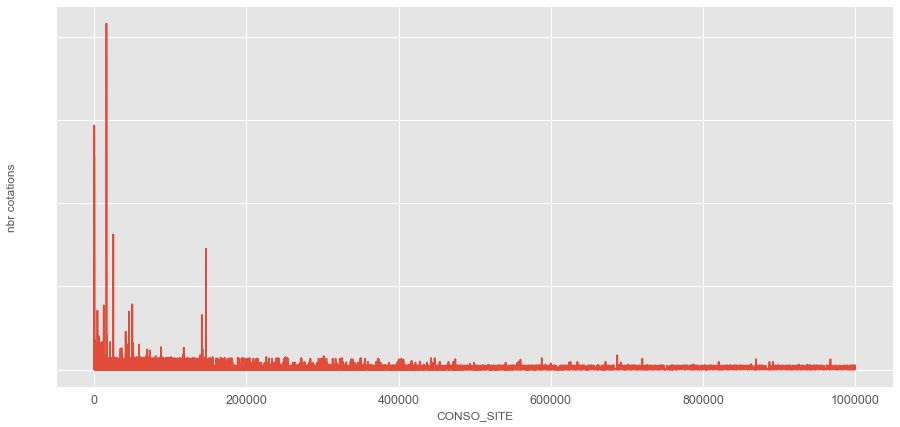
\includegraphics[width=1\textwidth]{image27.png}
     \caption{ Visualisation du nombre de négociations par rapport à l'évolution de la consommation}
    \label{fig:27}
\end{figure}

%%%%%%%%%%%%%%%%%%%%%%%%%%%%%%%%%%%%%%%%
{\bf Conclusion 3 :} Plus un site consomme moins le nombre de tours de négociations est faible.

\begin{itemize}
\item Mois de l’année
\end{itemize}

%%%%%%%%%%%%%%%% figure 28 %%%%%%%%%%%%%%

\begin{figure}[H]
	\centering
    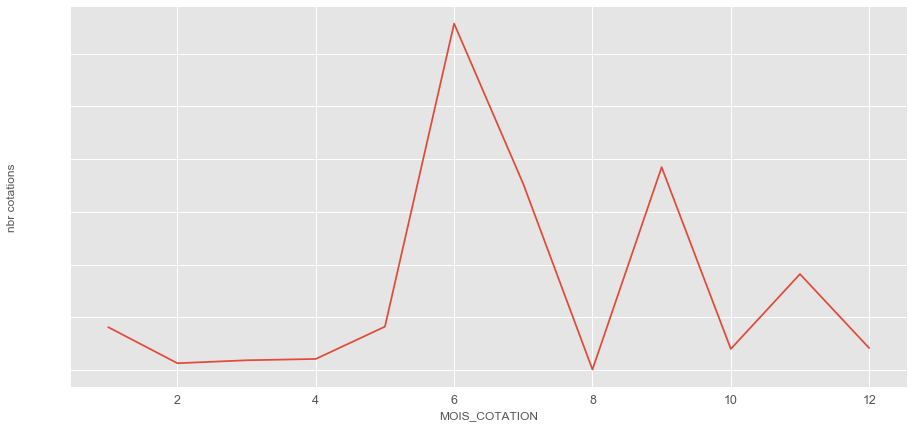
\includegraphics[width=1\textwidth]{image28.png}
     \caption{ Visualisation du nombre de négociations par rapport aux mois de l’année}
    \label{fig:28}
\end{figure}

%%%%%%%%%%%%%%%%%%%%%%%%%%%%%%%%%%%%%%%%
{\bf Conclusion 4 :} On remarque que les mois 6, 9 et 11 marquent les périodes les plus chargées en terme de négociations.

\underline{\bf Note:} Pour des raisons de confidentialité, les graphes servant à l’analyse ont été anonymisés.

-  Répartitions par rapport aux variables catégoriques :
\begin{itemize}
\item La nature de l’offre (compliquée ou pas)
\end{itemize}

%%%%%%%%%%%%%%%% figure 29 %%%%%%%%%%%%%%

\begin{figure}[H]
	\centering
    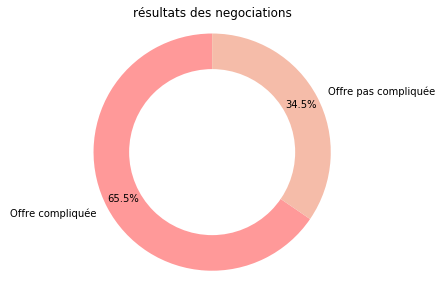
\includegraphics[width=0.7\textwidth]{image29.png}
     \caption{ Visualisation de la répartition de négociations par rapport à la nature de l'offre}
    \label{fig:29}
\end{figure}

%%%%%%%%%%%%%%%%%%%%%%%%%%%%%%%%%%%%%%%%
{\bf Conclusion 5 :} plus que la moitié des offres sont des offres compliquées.

\begin{itemize}
\item Score de liquidation judiciaire 
\end{itemize}

%%%%%%%%%%%%%%%% figure 30 %%%%%%%%%%%%%%

\begin{figure}[H]
	\centering
    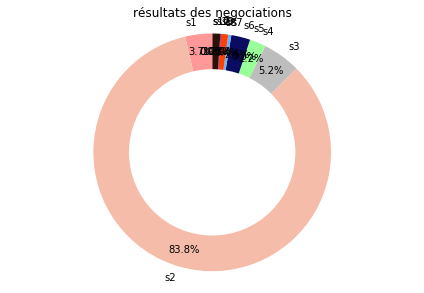
\includegraphics[width=0.65\textwidth]{image30.png}
     \caption{ Visualisation de la répartition de négociations par rapport au score de liquidation judiciaire}
    \label{fig:30}
\end{figure}

%%%%%%%%%%%%%%%%%%%%%%%%%%%%%%%%%%%%%%%%
{\bf Conclusion 6 :} La plupart des sites négociés sont des sites avec le score s1.

\begin{itemize}
\item Type client
\end{itemize}

%%%%%%%%%%%%%%%% figure 31 %%%%%%%%%%%%%%

\begin{figure}[H]
	\centering
    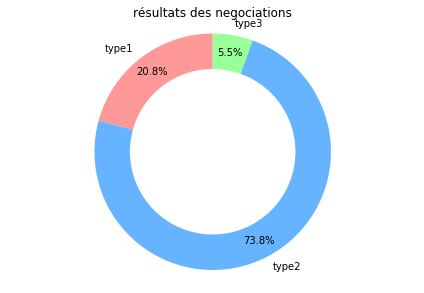
\includegraphics[width=0.7\textwidth]{image31.png}
     \caption{ Visualisation de la répartition de négociations par rapport au score de liquidation judiciaire}
    \label{fig:31}
\end{figure}

%%%%%%%%%%%%%%%%%%%%%%%%%%%%%%%%%%%%%%%%
{\bf Conclusion 7 :} Les clients de types 2 ont plus tendance à négocier que les autres types, ainsi que le type1 négocie mais son contrat sans partir chez les concurrents.

Ces graphes et d’autres qu’on a choisi de ne pas divulguer pour des raisons évidentes de confidentialité nous ont confirmé nos hypothèses ainsi que l’estimation de l’importance de nos variables. 

Cela nous a aidé à construire un vecteur de variables sur lequel on va appliquer nos algorithmes.

Le vecteur sera composé des variables suivantes:

{\bf V}= [	année de livraison,

forme de prix, 

nature du marché affaire, 

segment commercial ,

domaine de l’offre,

type client, 

score risque liquide du client , 

mode relève, 

consommation du  site,

type du contrat,

segment tarifaire du site,

durée du contrat, 

durée de validité de l’offre,

nombre d’occurence ou le site a été négocié,

date de négociation, 

complexité de l’offre ,

prix de marché ]

\subsection{Clustering de données et segmentation des clients } 

Dans ce chapitre, les algorithmes de cluster seront testés et leurs performances seront mesurées. La meilleure méthode de cluster de travail sera utilisée pour déterminer les segments. Le chapitre suivant se soldera par une évaluation des segments.

{\bf PCA et réduction de bruit:}

Avant d’appliquer PCA le plot des données a donné le résultat suivant:
%%%%%%%%%%%%%%%% figure 32 %%%%%%%%%%%%%%

\begin{figure}[H]
	\centering
    
\includegraphics[width=0.7\textwidth]{image32.png}
     \caption{ Plot avant PCA}
    \label{fig:32}
\end{figure}

%%%%%%%%%%%%%%%%%%%%%%%%%%%%%%%%%%%%%%%%
en appliquant PCA, le résultat est le suivant:
%%%%%%%%%%%%%%%% figure 33 %%%%%%%%%%%%%%

\begin{figure}[H]
	\centering
    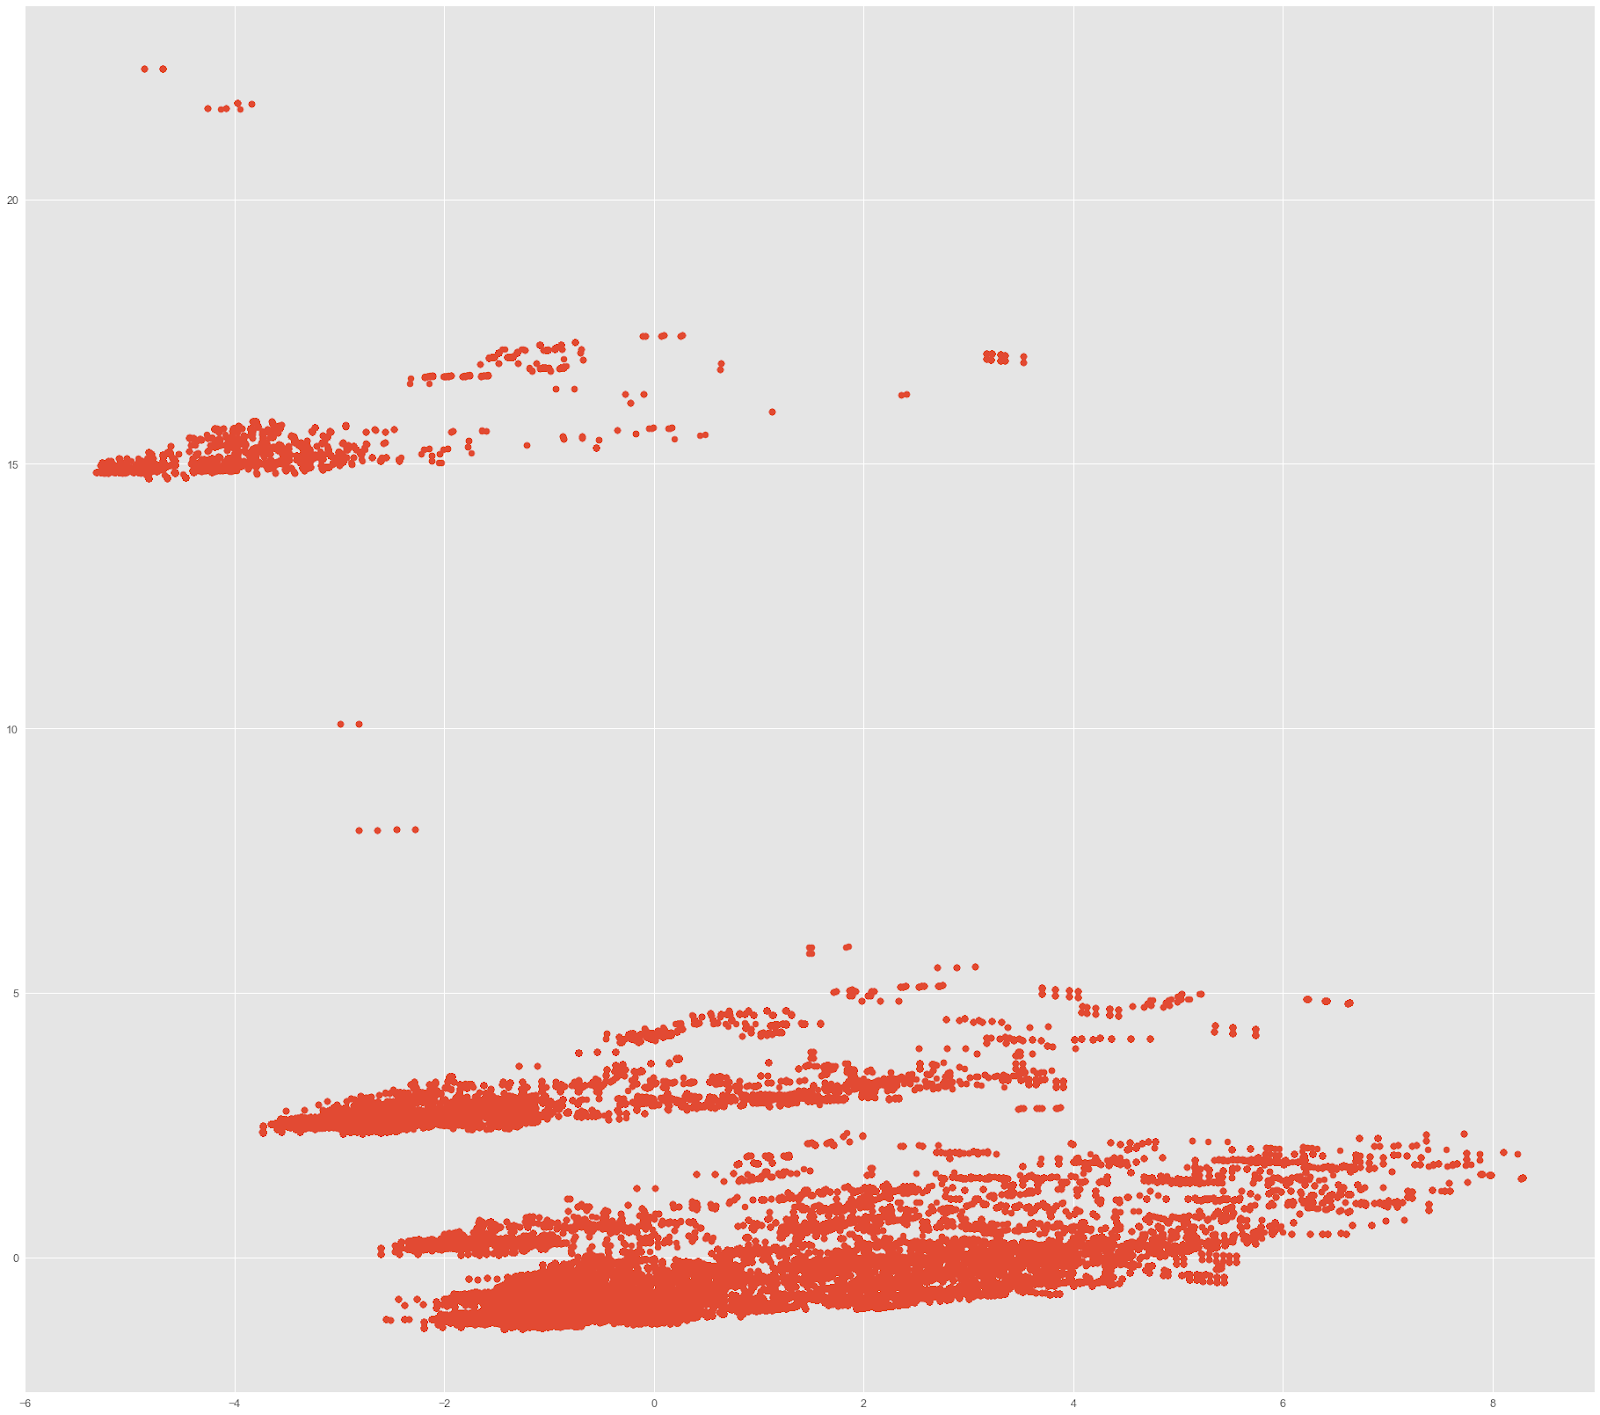
\includegraphics[width=0.7\textwidth]{image33.png}
     \caption{ Plot après PCA}
    \label{fig:33}
\end{figure}

%%%%%%%%%%%%%%%%%%%%%%%%%%%%%%%%%%%%%%%%
{\bf PCA} nous a  aidé à avoir une meilleure présentation des données avec moins de bruit.
Par la suite, nos données sont bien prêtes pour l’application des algorithmes.

{\bf Déterminer le nombre optimal des clusters}

L'inconvénient des algorithmes de clustering est le nombre de clusters qui doit être donné à l'avance ce qui n’est pas connu pour notre cas. Par conséquent, Il doit être recherché avec les méthodes de validation données. Notamment un processus appelé Elbow Criterion. Le critère du coude est une règle empirique courante pour déterminer le nombre de clusters à choisir.

Le critère du coude indique qu'il faut choisir un certain nombre de clusters de sorte que l'ajout d'un autre cluster n'ajoute pas suffisamment d'informations. 
Plus précisément, en réalisant un graphique d’une mesure de validation expliquée par les clusters par rapport au nombre de clusters, les premiers clusters ajouteront beaucoup d'informations (expliquent beaucoup de variance), mais à un certain point le gain marginal diminuera, donnant un angle au graphique ( le coude “Elbow”).

Le nombre de clusters est choisi à ce stade, d'où le "critère du coude". Ce "coude" ne peut pas toujours être identifié sans ambiguïté.

{\bf K-means et méthode elbow:}

On a appliqué la méthode Elbow avec le K Means qui nous a donné un nombre maximum de 20 clusters possibles comme le montre le graphique suivant:

%%%%%%%%%%%%%%%% figure 34 %%%%%%%%%%%%%%

\begin{figure}[H]
	\centering
    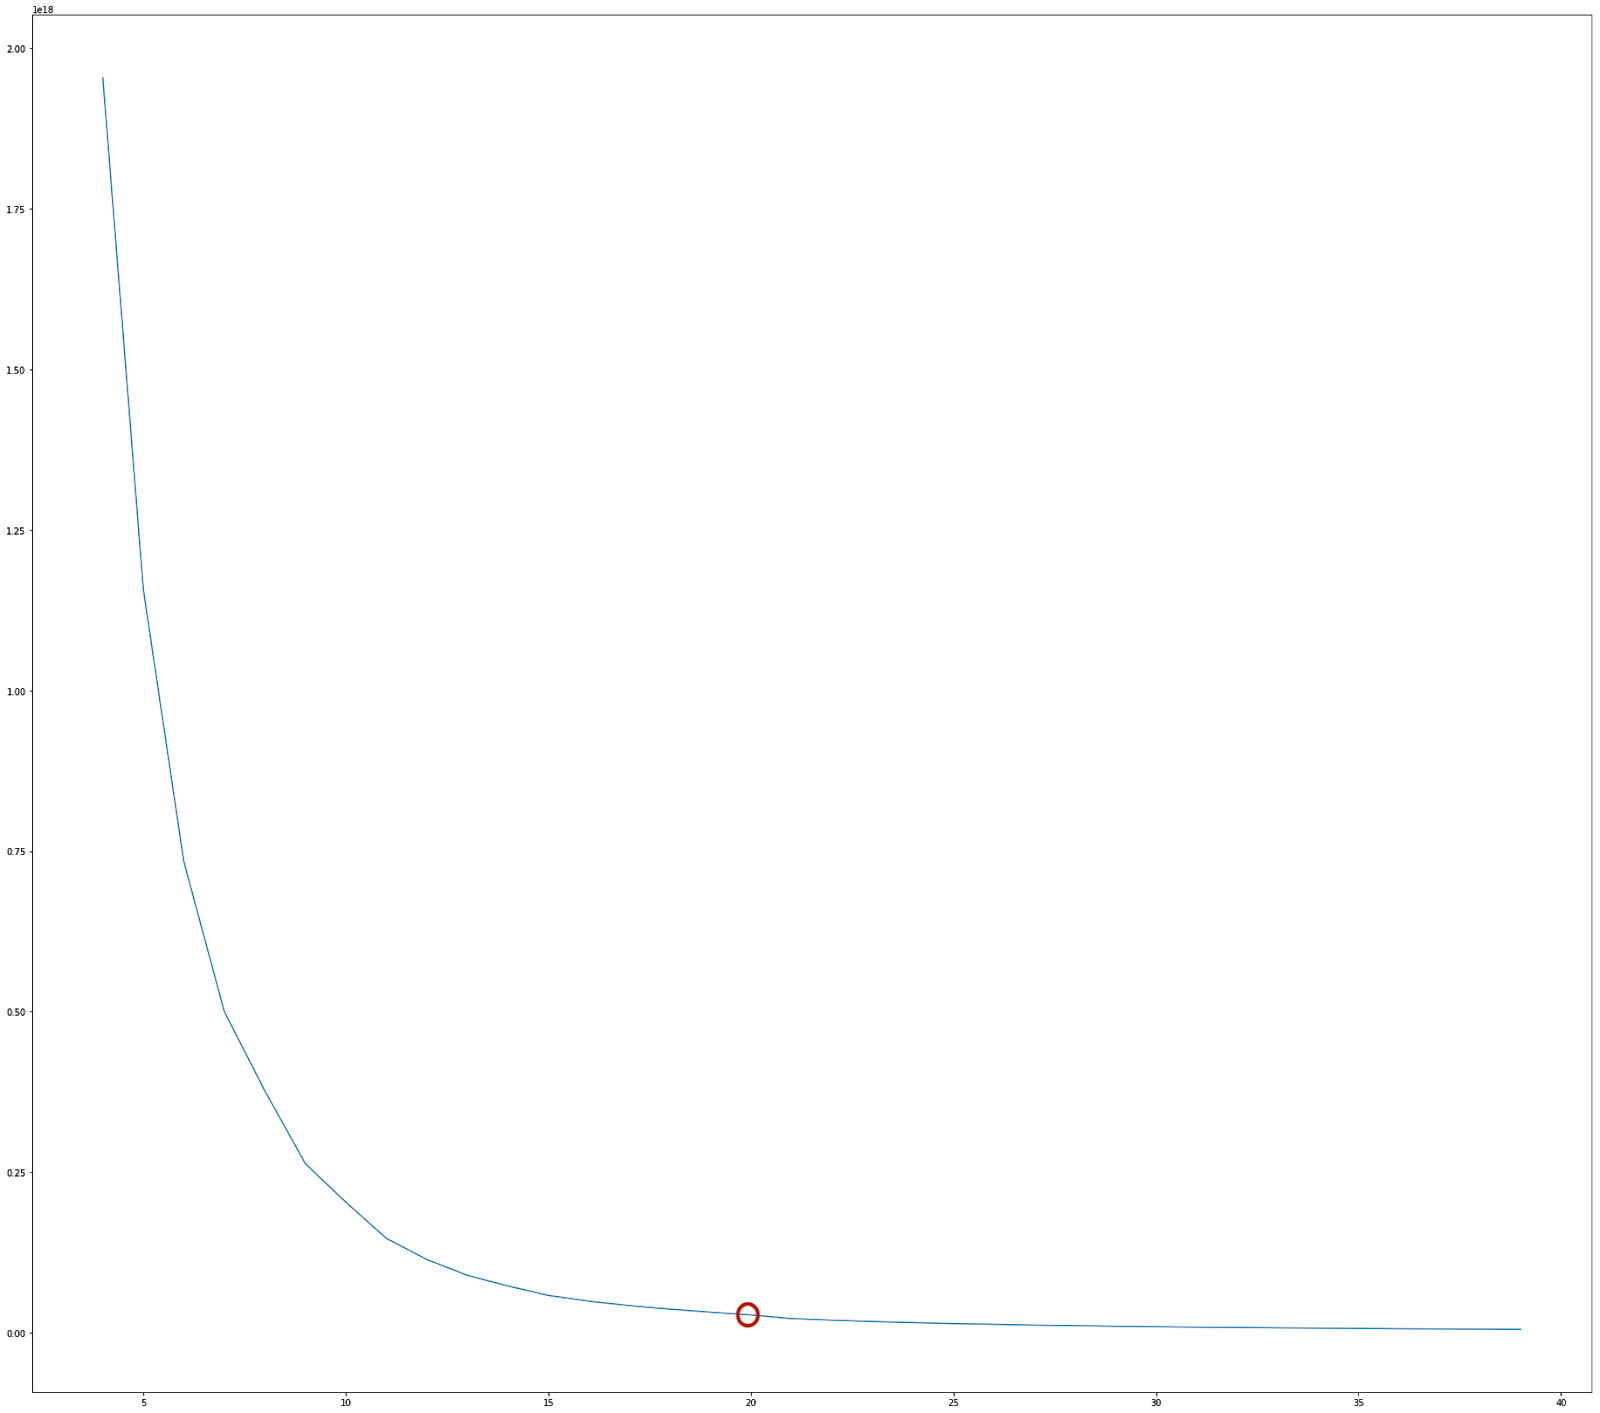
\includegraphics[width=0.7\textwidth]{image34.png}
     \caption{ Définition du nombre des clusters par la méthode elbow}
    \label{fig:34}
\end{figure}

%%%%%%%%%%%%%%%%%%%%%%%%%%%%%%%%%%%%%%%%
Maintenant vient l’importance du rôle de la datavisualisation pour nous aider à identifier le nombre correcte de clusters.

Avec 20 clusters on a eu le résultat suivant :

%%%%%%%%%%%%%%%% figure 35 %%%%%%%%%%%%%%

\begin{figure}[H]
	\centering
    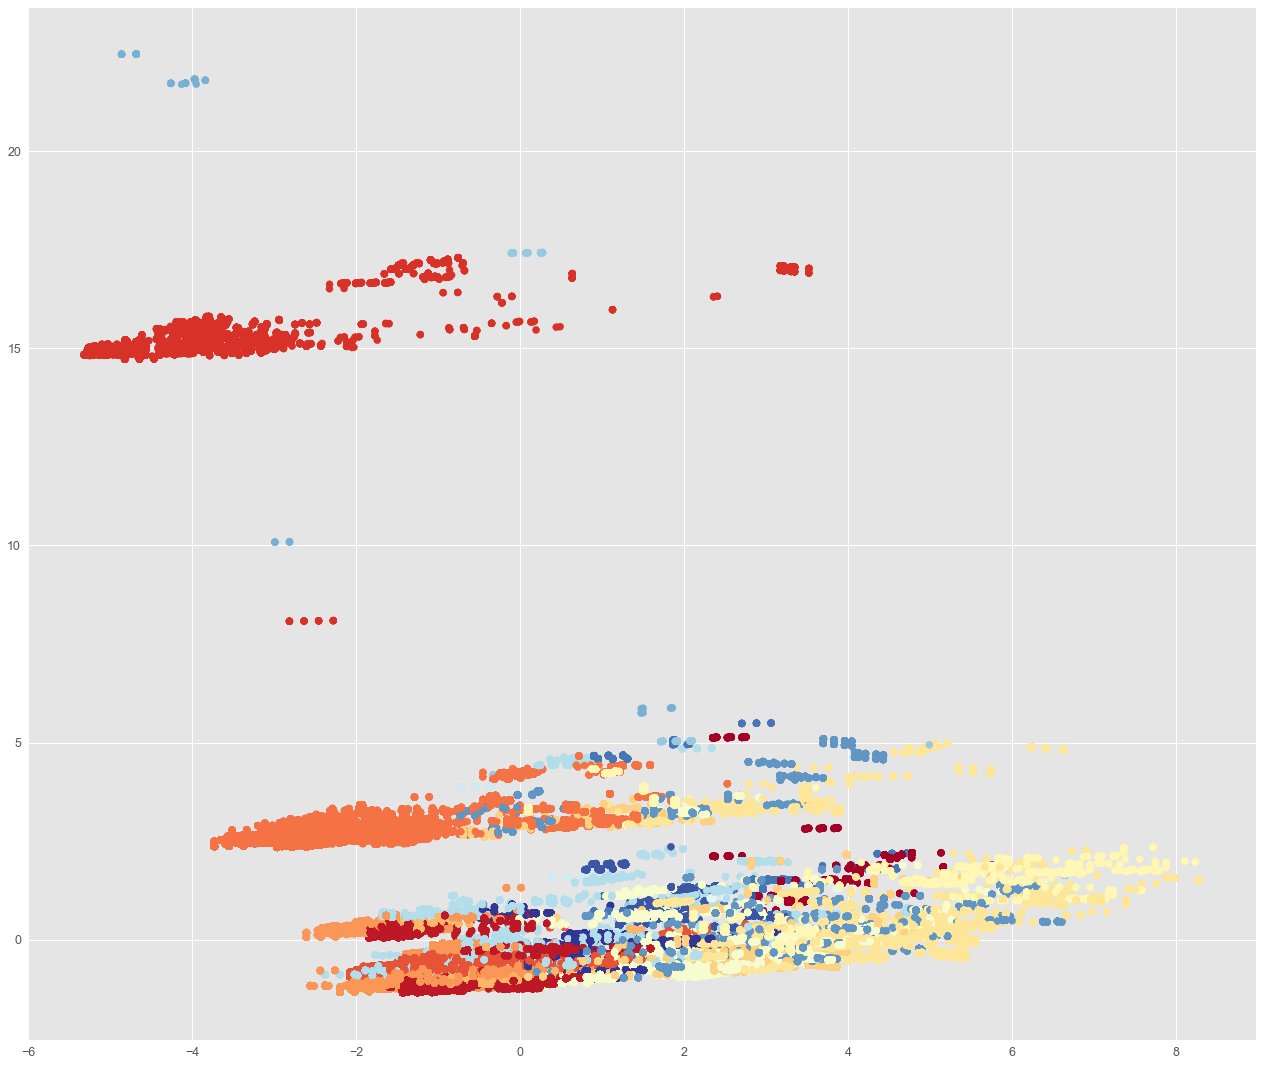
\includegraphics[width=0.7\textwidth]{image35.png}
     \caption{ Plot K means avec 20 clusters}
    \label{fig:35}
\end{figure}

%%%%%%%%%%%%%%%%%%%%%%%%%%%%%%%%%%%%%%%%

Alors qu’avec 8 clusters nous avons le résultat suivant :

%%%%%%%%%%%%%%%% figure 36 %%%%%%%%%%%%%%

\begin{figure}[H]
	\centering
    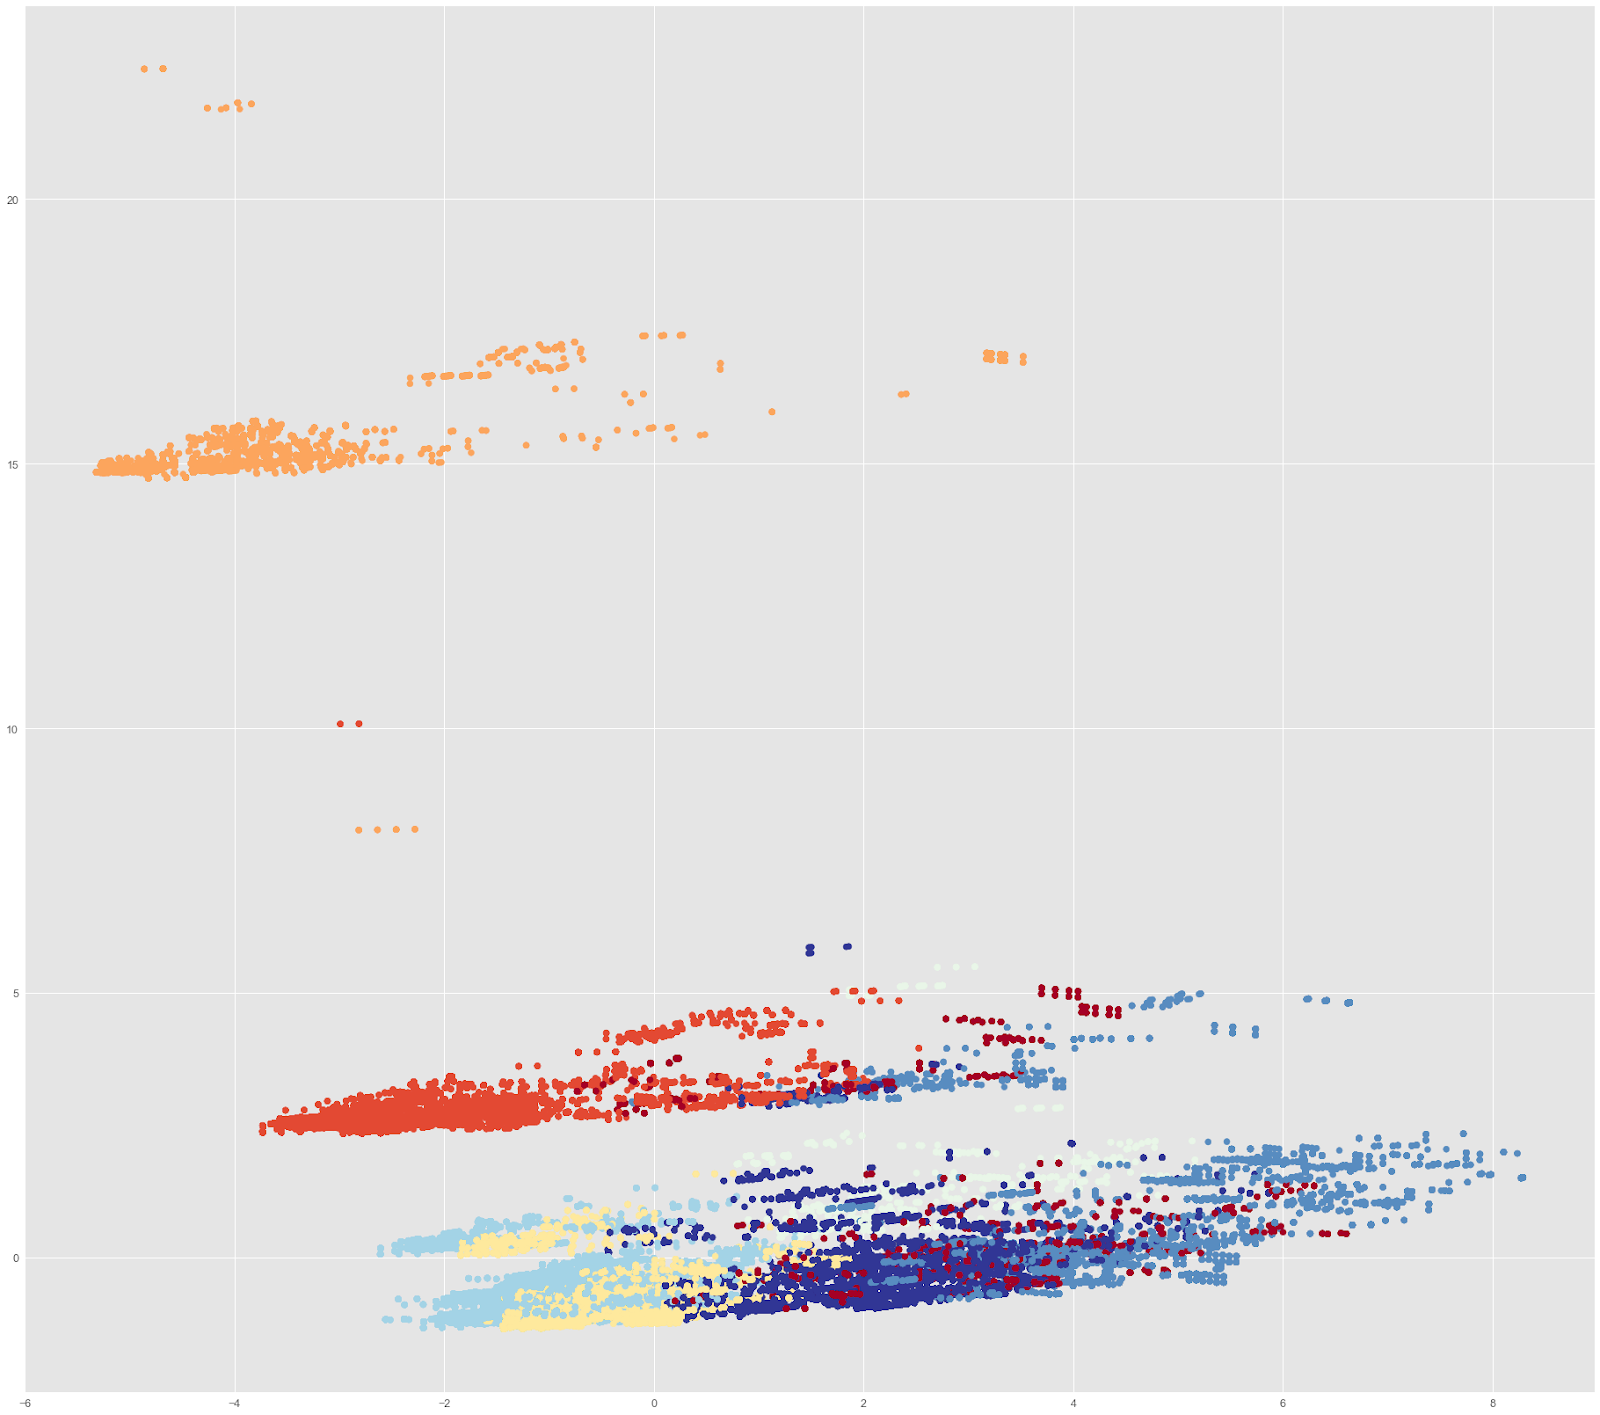
\includegraphics[width=0.7\textwidth]{image36.png}
     \caption{ Plot K means avec 8 clusters}
    \label{fig:36}
\end{figure}

%%%%%%%%%%%%%%%%%%%%%%%%%%%%%%%%%%%%%%%%

On constate qu’il faut diminuer le nombre de clusters.

avec 5 clusters :
%%%%%%%%%%%%%%%% figure 37 %%%%%%%%%%%%%%

\begin{figure}[H]
	\centering
    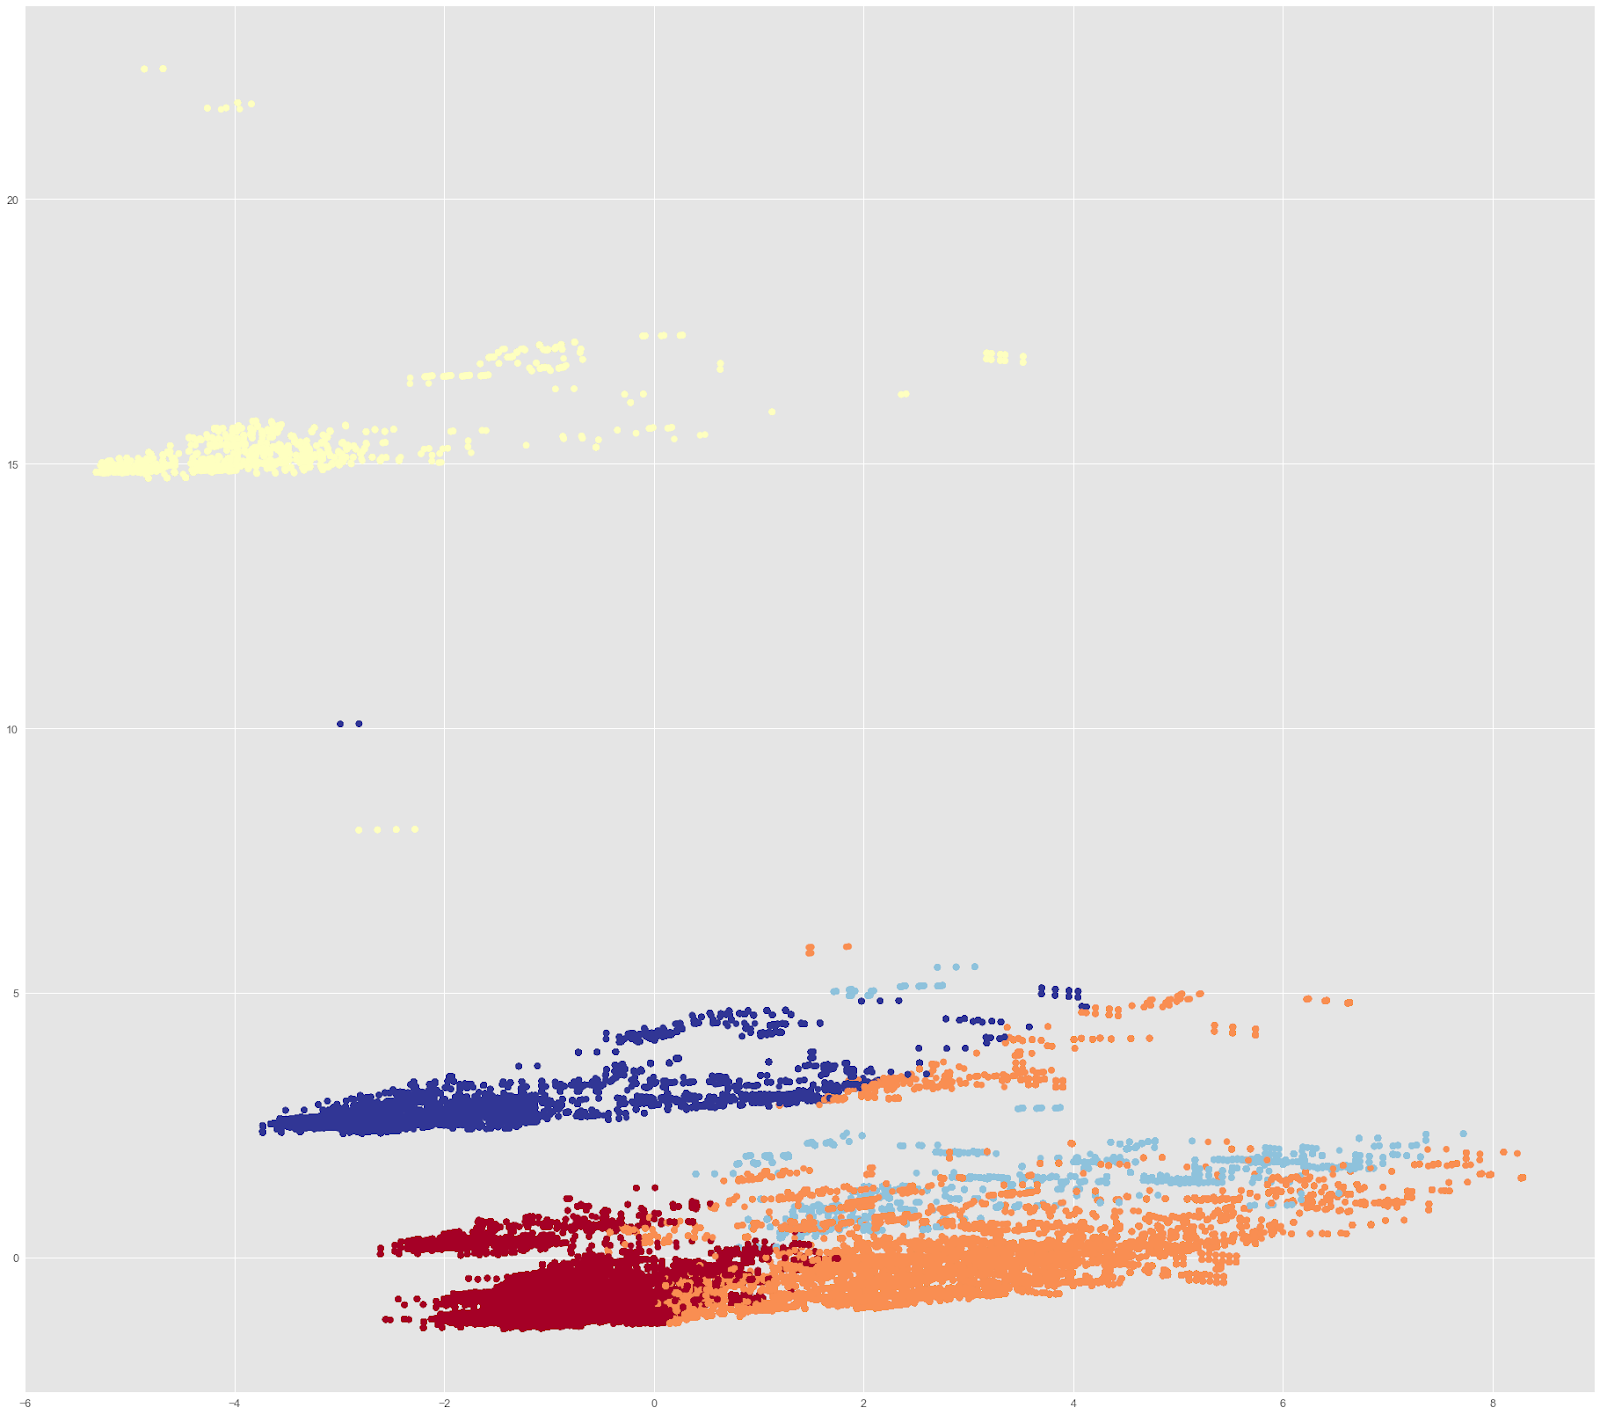
\includegraphics[width=0.7\textwidth]{image37.png}
     \caption{ Plot K means avec 5 clusters}
    \label{fig:37}
\end{figure}

%%%%%%%%%%%%%%%%%%%%%%%%%%%%%%%%%%%%%%%%

avec 4 clusters:
%%%%%%%%%%%%%%%% figure 38 %%%%%%%%%%%%%%

\begin{figure}[H]
	\centering
    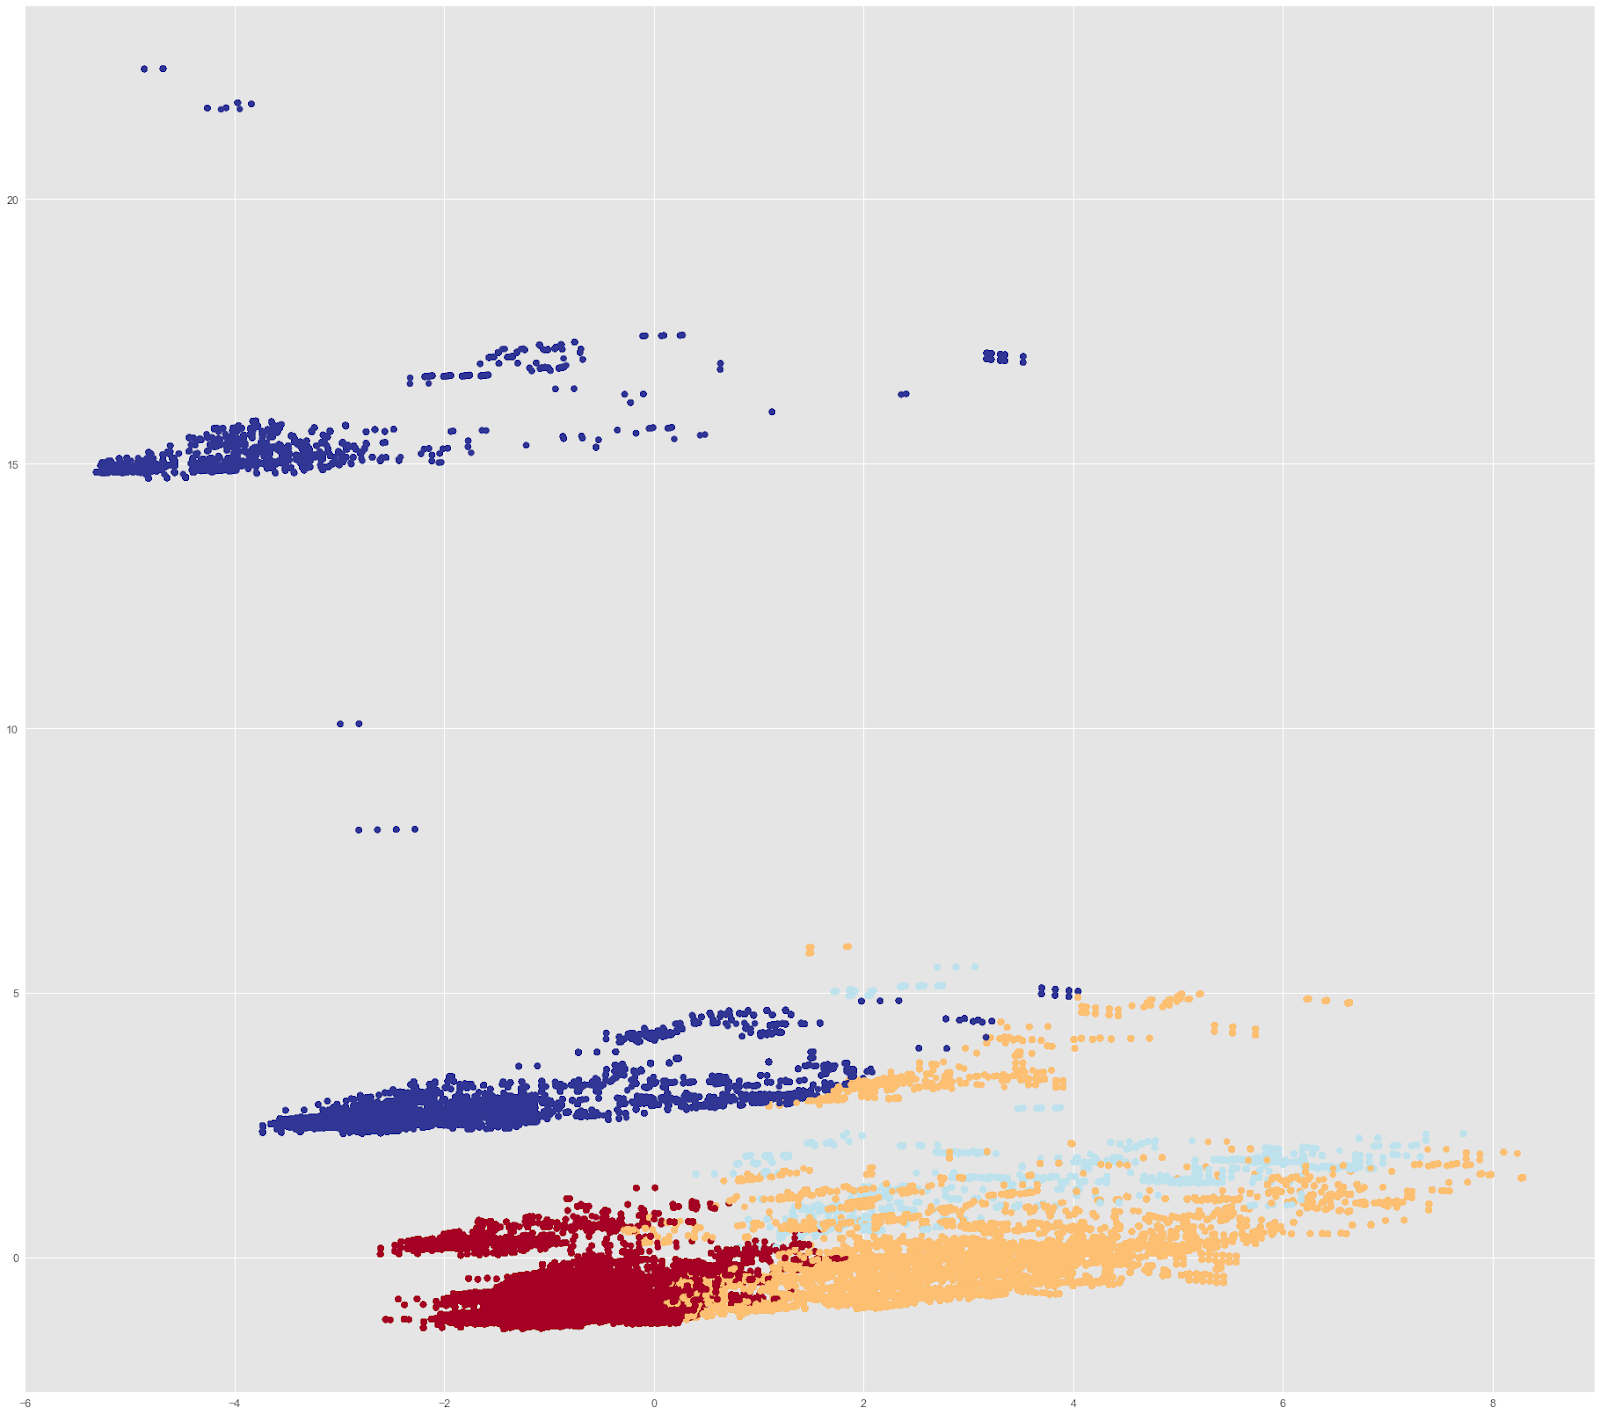
\includegraphics[width=0.7\textwidth]{image38.png}
     \caption{ Plot K means avec 4 clusters}
    \label{fig:38}
\end{figure}

%%%%%%%%%%%%%%%%%%%%%%%%%%%%%%%%%%%%%%%%

La datavisualisation nous a confirmé que le nombre correcte de clusters est 5. Donc nos clients peuvent être regroupés en 5 segments différents.


Afin d’avoir une bonne vision des clients. il faut étudier chaque cluster séparément et identifier ses caractéristiques et finalement projeter chaque client dans cette segmentation si besoin.

Pour étudier chaque cluster séparément on va appliquer l’algorithme de clustering K-means dans le logiciel WEKA, le logiciel libre d'apprentissage automatique qui contient une collection d'outils de visualisation et d'algorithmes pour l'analyse des données et la modélisation prédictive.

Le nombre de chaque membre du cluster et également les valeurs moyennes de chaque variable dans les clusters sont affichés dans le tableau ci dessous:

%%%%%%%%%%%%%%%% figure 39 %%%%%%%%%%%%%%

\begin{figure}[H]
	\centering
    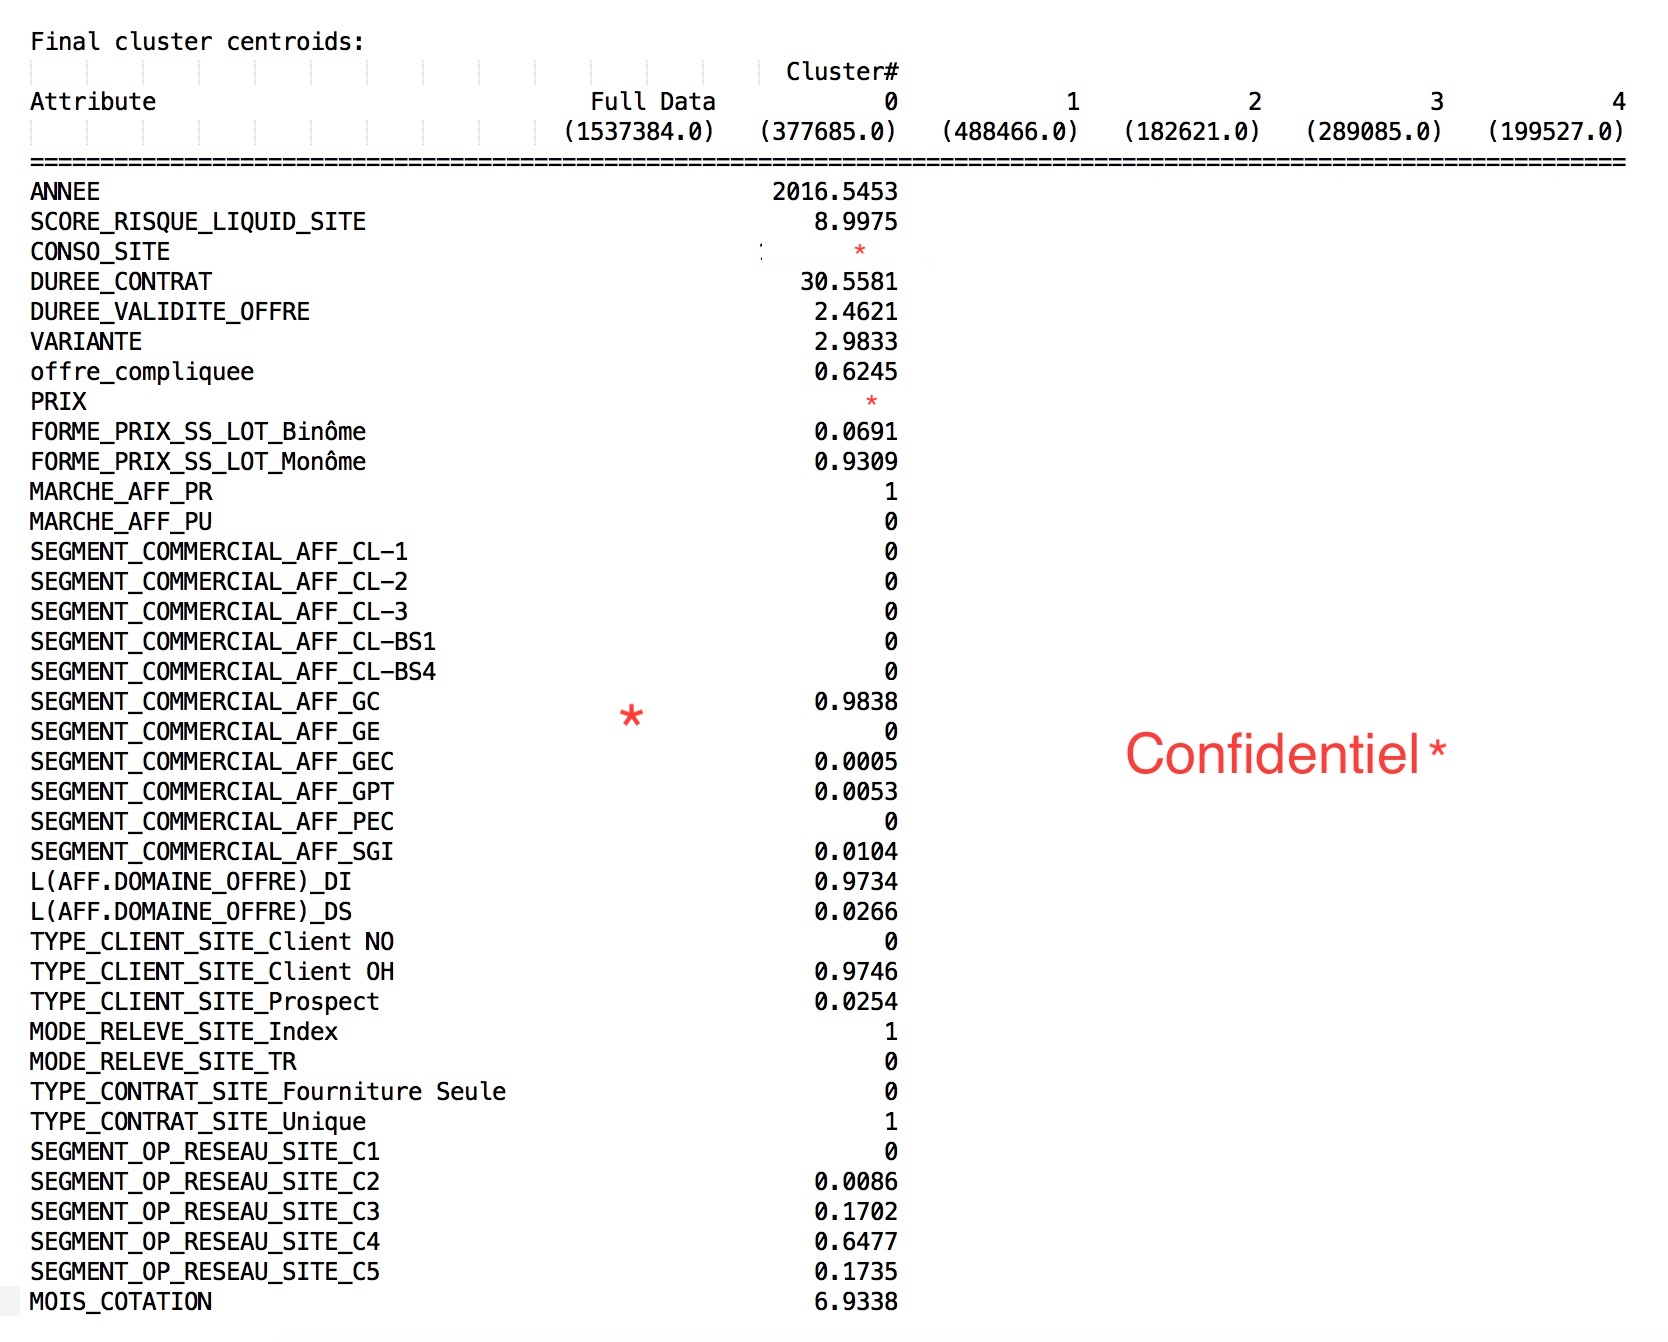
\includegraphics[width=1\textwidth]{image39.png}
     \caption{Final cluster centroids}
    \label{fig:39}
\end{figure}

%%%%%%%%%%%%%%%%%%%%%%%%%%%%%%%%%%%%%%%%


Comment interprétons-nous ces résultats? ce tableau nous montre comment chaque cluster se réunit, avec un "1" signifiant que tout le monde partage la même valeur et un "0" signifiant que tout le monde dans ce cluster a une valeur de zéro pour cet attribut. 
Les nombres représentent la valeur moyenne de tous les membres du cluster. Chaque cluster nous montre un type de comportement chez nos clients, à partir duquel nous pouvons commencer à tirer quelques conclusions:

{\bf Cluster 0:} Ce segment rassemble les petits sites avec des relevés tous les 6 mois des clients du marché Privé qui appartiennent au segment commercial GC et qui ont un contrat unique et qui ont négocié en moyenne 2 fois depuis leur souscription avec une durée de contrat moyenne à 30 mois et qui ont tendance de négocier quand le prix de marché évolue.

{\bf Cluster 1:} Ce segment rassemble les petits sites aussi toujours marché privé mais qui appartiennent au segment commercial GE qui ont l’habitude de négocier en moyenne 6 fois avec une durée de contrat moyenne de 32 mois et qui choisissent des offres avec des options (0,73>0,65 offre compliquée par rapport à la moyenne ) et par contre qui ne négocient pas toujours quand le prix de marché évolue.

{\bf Cluster 2:} Ce segment par contre rassemble les sites publics et privés qui ont des courbes de charge (TR) et qui appartient au segment commercial GE et GC et au segment tarifaire C2 avec une habitude de négoce de 5 fois en moyenne et durée de contrat moyenne de 29 mois 

{\bf Cluster 3:} Ce segment rassemble les petits sites (index) qui ont été coté en 2018 avec les durées de contrat les plus courtes et qui ont l’habitude de négocier 4 fois depuis leur souscription. la plupart de ces sites sont privés et appartiennent au segment commercial et qui ont des nouvelles offres NO avec des segment tarifaire C3,C4 et C5.

{\bf Cluster 4:} Ce segment rassemble les petits sites, avec comme moyenne de consommation la plus petite par rapport aux autres segment, qui n’ont pas l’habitude de négocier (moyenne une fois depuis leur souscription ) et qui sont entre offre historique et prospect et qui appartiennent au segment commercial CL-1 et qui ont une durée de validité de l'offre plus importante.

Caractéristique communes entre les 5 segmentations:

→ Tous les clients ont tendance à négocier pendant la période d’été ( entre mois 6 et 7) 

→ La plupart des clients passent par le montage d’offre

→ Tous les sites payent bien d’une manière générale ( score risque à 8 qui signifie 0 )

Les données sont distribuées sur les clusters comme suit:


\begin{center}
\begin{tabular}{|p{3cm}|p{3cm}|p{3cm}|}
\hline
 
num Cluster & nombre d’instances & Pourcentage \\
  \hline
  
0& 377685 & 25\% \\
  \hline
1 & 488466 & 32\% \\
  \hline

2 & 182621 & 12\%\\
 
 
3 &289085 & 19\%\\
 \hline
4 &199527 &13\%\\
  \hline
\end{tabular}
\end{center}
%%%%%%%%%%%%%%%% figure 40 %%%%%%%%%%%%%%
\begin{figure}[H]
	\centering
    
     \caption{ distribution des données sur les clusters}
    \label{fig:40}
\end{figure}

%%%%%%%%%%%%%%%%%%%%%%%%%%%%%%%%%%%%%%%%
La construction du model a pris sur Weka : 36.9 seconds


\subsection{Conclusion et Perspectives}
Ce mémoire a proposé une étude de cas professionnelle, avec une segmentation concrète des clients comme première étape vers la réponse à l'énoncé de la problématique de base (Comment les données et le data mining pourraient aider un fournisseur de l’énergie à anticiper une négociation ?).

La segmentation des clients est une méthode de regroupement des clients basée sur les similitudes qu'ils partagent en ce qui concerne toutes les dimensions, qu'il s'agisse des besoins des clients, des préférences de canal, de l'intérêt pour certaines fonctionnalités, de la rentabilité des clients, etc. 

dans le cas où les données ne sont pas complètes, elle peut servir comme une bonne première  étape pour faire de la prédiction si on couple les données avec une base de règles issue de la bonne compréhension du domaine et des différents facteurs influençants ce dernier.

Donc nous pouvons supposer sans risque que le Data Mining puisse aider les fournisseurs d’énergie à avoir une meilleure vision de leurs clients ainsi que d’identifier certaines négociations, mais pas toutes, en utilisant des algorithmes de clustering et prédictions binaires communes. 

Alors oui, il soutient les fournisseurs de l'énergie, mais il est trop limité pour le proposer comme une solution "anti-départs" surtout que le marché de l'énergie ainsi que l’achat industriel sont plus complexes comme ce qui a été décrit dans la première partie de ce mémoire.

En ce qui concerne le Process Data Mining, il s'agit d'une gamme de recherche complète à explorer, qui nécessiterait la même quantité ou même plus de recherches et d'expériences pour obtenir le même niveau d'information. Mais connaissant les limites de Data Mining, il apparaît comme la clé d'une meilleure réponse à notre problématique.


\subsubsection{Limites:}
Les méthodes proposées nécessitent de nombreuses données client pour être validées de manière adéquate.

Dans cette étude, nous avions des informations limitées et incomplètes sur les clients, leur historique de négociation et surtout que les données qu’on a pu récupérer ne répondaient pas à notre besoin mais à une logique métier.
En raison de notre base de données incomplète et incorrecte ainsi que le temps consacré pour le traitement de cette dernière, nous n'avons pas pu analyser les autres méthodes de segmentation des clients et, par conséquent, il était impossible de comparer nos méthodes proposées avec d'autres méthodes.


\subsubsection{Perspectives:}
Je proposerai par la suite de suivre après cette étude les points suivants:

\begin{itemize}
\item Continuer notre étude afin d'établir une bonne base de règles permettant d'influencer les négociations

\item Prédire les moment où les prix de marché peuvent augmenter et projeter sur le résultat du clustering, pour identifier les segments qui réagissent à cette évolution du marché.

\end{itemize}

\newpage
\section{BIBLIOGRAPHIE:}
\begin{itemize}
    \item [Durand 1995] Jean-Paul Durand,(1995), Le Langage des Achats, Éd. Méthodes et stratégies
    \item [Gorunescu 2011] Gorunescu, F. (2011). Data Mining: Concepts, models and techniques (Vol. 12). Springer Science and Business Media.
    \item [Bounsaythip 2001] Bounsaythip, C. and Rinta-Runsala, E.,(2001), Overview of Data Mining for Customer Behavior Modeling. Research report TTE1-2001-18, VTT Information Technology 
    \item [PINON 2015] Xavier PINON et Thomas VERON, (2015), Le marché de détail de l’énergie : la concurrence en action dans l’électricité et le gaz by ISBN: 978-2-343-05447-6
    \item [Fröhlich, 1997] https://www.nnwj.de/kohonen-feature-map.html
    \item [Brownlee 2014] http://machinelearningmastery.com/an-introduction-to-feature-selection/, Brownlee 2014
    \item [C. Duby, S. Robin] C. Duby, S. Robin, cours Analyse en Composantes Principales , AgroParisTech http://www2.agroparistech.fr/IMG/pdf/AnalyseComposantesPrincipales-AgroParisTech.pdf
     \item [Ahmet Cece,2016] Ahmet Cece, (2016), Brief Visual Explanation of PCA http://www.ahmetcecen.tech/blog/class/2016/10/04/PCA/
     \item [Vesanto \& Alhoniemi, 2000] Vesanto \& Alhoniemi, (2000) Clustering of the auto-organizing map
    \item [1]: Partitional Clustering, http://www.sthda.com/english/articles/27-partitioning-clustering-essentials/89-clara-clustering-large-applications
    \item [Vesanto,2006],(2006) Vesanto, Using SOM in Data mining, 2000, Tan, Steinbach et Kumar
    \item [2], http://www.sthda.com/english/articles/28-hierarchical-clustering-essentials
    \item [Tan, Steinbach, \& Kumar, 2006],Tan, Steinbach, \& Kumar,Clustering de la carte auto-organisatrice 2006
    \item [Arnborg, 2008]
    \item [Jain, Murty, \& Flynn, 1999] Jain, Murty, \& Flynn, 1999 Data Clustering: A Review
    \item [Jain et Dubes, 1988] Jain et Dubes, 1988, Algorithms for Clustering Data
    \item Berry, M.,\& Linoff, G. S. (2004). Data Mining Techniques: For Marketing,Sales, and Customer Relationship Management. Indianapolis, Indiana,Unites States of America: Wiley Publishing.
   \item [Tan, Steinbach et Kumar, 2006],Tan, P.-N., Steinbach, M., \& Kumar, V. (2006). Introduction to data mining. Boston, United States of America: Pearson Education, Inc.
   \item [Kohonen, Self-organizing map, 1995],Kohonen, T. (1995). Self-organizing map. Berlin: Springer.
   \item [Kiang, Hu et Fisher, 2006],Kiang, M. Y., Hu, M. Y., \& Fisher, D. M. (October 2006). An extended self-organizing map network for market segmentation—a telecommunication example. Decision Support Systems, pp. 36-47.
   \item [ Vellido, Lisboa et Meehan, 1999] Vellido, A., Lisboa, P. J.,\& Meehan, K. (1999). Segmentation of the on-line
shopping market using neural network. Expert Systems with Applications
   \item [Hsieh, 2004] Hsieh,(November 2004). An integrated data mining and behavioral scoring model for analyzing bank customers. Expert Systems with
Applications 
    \item [Merkevičius, Garšva et Simutis, 2004] Merkevičius, E., Garšva, G., \& Simutis, R. (2004). Forecasting of credit classes with the self-organizing maps. Information Technology And Control
     \item [Cortes \& Vapnik, 1995] Cortes\& Vapnik, V. (1995). Support-vector networks. Machine Learning
     \item [Spoustova 2009] Hajič, J., Raab, J., \& Spousta, M. (2009, March). Semi-supervised training for the averaged perceptron POS tagger. In Proceedings of the 12th Conference of the European Chapter of the Association for Computational Linguistics. Association for Computational Linguistics.
     \item [Herbrich 2001]Herbrich, R., Graepel, T., \& Campbell, C. (2001). Bayes point machines. Journal of Machine Learning Research, 1(Aug)
     \item [Coadou 2015] Coadou, Y. (2016, May). Boosted decision trees. In IN2P3 School of Statistics 2016.
     \item [Chen 2005]Chen, X. W., \& Liu, M. (2005). Prediction of protein–protein interactions using random decision forest framework. Bioinformatics
     \item [King 2001] King, G., \& Zeng, L. (2001). Logistic regression in rare events data. Political analysis 
     \item [Rowley 1998]Rowley, H. A., Baluja, S., \& Kanade, T. (1998). Neural network-based face detection. IEEE Transactions on pattern analysis and machine intelligence
      \item [Hearst 1998] Hearst, M. A., Dumais, S. T., Osuna, E., Platt, J., \& Scholkopf, B. (1998). Support vector machines. IEEE Intelligent Systems and their applications
     \item [Xi Zhang X. et Tang Y, 2006] Xi Zhang and Yu Tang, (2006), Customer Perceived E-service Quality in Online Shopping. Master Thesis, Lulea University, Department of Business Administration and Social Sciences Division of Industrial marketing and e-commerce.
     \item [Madani, S., 2009]Samira Madani, (2009), Mining Changes in Customer Purchasing Behavior - a Data Mining Approach. Master Thesis, Lulea University, Department of Business Administration and Social Sciences Division of Industrial marketing and e-commerce.
     \item [Wang C. et Wang Zh., 2006] Hai Wang, and Shouhong Wang (2006), A Purchasing Sequences Data Mining Method for Customer Segmentation, IEEE Conference on Service Operations and Logistics, and Informatics
     \item [Nosrati, 2008]LalehNosrati, (2008), The Impact of Website Quality on Customer Satisfaction. A Research on Iranian Online Bookstores, Master Thesis, Lulea University, Department of Business Administration and Social Sciences Division of Industrial marketing and e-commerce.
     \item [Yin, 2003, p.5] Yin, R. K. (2003), Case study Research Design and Methods(3rd ed.) California: Sage Publications
     \item [Benbasa et al, 1987]Izak Benbasat, David K. Goldstein and Melissa Mead (1987) The case research strategy in studies of information systems. MIS Quarterly
     \item [Huaping Gong, Qiong Xia, 2009]Huaping Gong, Qiong Xia (2009), Study on Application of Customer Segmentation Based on Data Mining Technology, IEEE Conference on ETP International Conference on Future Computer and Communication
     \item [Cheng Li, 2008] Cheng Li (2008) Research on Segmentation implementation process of air cargo customer based on Data Mining, IEEE 4th International Conference on Wireless Communications,Networking and Mobile Computing
\end{itemize}


\end{document}
